\documentclass[12pt]{beamer}
\newenvironment{ConCodigo}[1]
  {\begin{frame}[fragile,environment=ConCodigo]{#1}}
  {\end{frame}}
\graphicspath{{Imagenes/}{../Imagenes/}}
\usepackage[utf8]{inputenc}
\usepackage[spanish]{babel}
\usepackage{hyperref}
\usepackage{etex}
\reserveinserts{28}
\usepackage{amsmath}
\usepackage{amsthm}
\usepackage{mathtools}
\usepackage{multicol}
\usepackage{multirow}
\usepackage{tabulary}
\usepackage{booktabs}
\usepackage{nccmath}
\usepackage{biblatex}
\usepackage{epstopdf}
\usepackage{graphicx}
%\usepackage{enumitem,xcolor}
\usepackage{siunitx}
\sisetup{scientific-notation=true}
%\usepackage{fontspec}
\usepackage{lmodern}
\usepackage{float}
\usepackage[format=hang, font=footnotesize, labelformat=parens]{caption}
\usepackage[autostyle,spanish=mexican]{csquotes}
\usepackage{standalone}
\usepackage{blkarray}
\usepackage{algorithm}
\usepackage{algorithmic}
\usepackage{tikz}
\usepackage[siunitx]{circuitikz}
\usetikzlibrary{arrows,patterns,shapes}
\usetikzlibrary{decorations.markings}
\usetikzlibrary{arrows}
\usepackage{color}
\usepackage{xcolor}
%\usepackage{beton}
%\usepackage{euler}
%\usepackage[T1]{fontenc}
\usepackage[sfdefault]{roboto}  %% Option 'sfdefault' only if the base font of the document is to be sans serif
\usepackage[T1]{fontenc}
\renewcommand*\familydefault{\sfdefault}
\DeclareGraphicsExtensions{.pdf,.png,.jpg}
\usepackage{hyperref}
\renewcommand {\arraystretch}{1.5}
\newcommand{\python}{\texttt{python}}
\usefonttheme[onlymath]{serif}
\setbeamertemplate{navigation symbols}{}
\usetikzlibrary{patterns}
\usetikzlibrary{decorations.markings}
\tikzstyle{every picture}+=[remember picture,baseline]
%\tikzstyle{every node}+=[inner sep=0pt,anchor=base,
%minimum width=2.2cm,align=center,text depth=.15ex,outer sep=1.5pt]
%\tikzstyle{every path}+=[thick, rounded corners]
\setbeamertemplate{caption}[numbered]
\newcommand{\ptm}{\fontfamily{ptm}\selectfont}
%Se usa la plantilla Warsaw modificada con spruce
\mode<presentation>
{
  \usetheme{Warsaw}
  \setbeamertemplate{headline}{}
  \useoutertheme{default}
  \usecolortheme{seahorse}
  \setbeamercovered{invisible}
}
% \AtBeginSection[]
% {
% \begin{frame}<beamer>{Contenido}
% \normalfont\mdseries
% \tableofcontents[currentsection]
% \end{frame}
%}

\usepackage{courier}
\usepackage{listingsutf8}
\usepackage{listings}
\usepackage{xcolor}
\usepackage{textcomp}
\usepackage{color}
\definecolor{deepblue}{rgb}{0,0,0.5}
\definecolor{brown}{rgb}{0.59, 0.29, 0.0}
\definecolor{OliveGreen}{rgb}{0,0.25,0}
% \usepackage{minted}

\DeclareCaptionFont{white}{\color{white}}
\DeclareCaptionFormat{listing}{\colorbox{gray}{\parbox{0.98\textwidth}{#1#2#3}}}
\captionsetup[lstlisting]{format=listing,labelfont=white,textfont=white}
\renewcommand{\lstlistingname}{Código}


\definecolor{Code}{rgb}{0,0,0}
\definecolor{Keywords}{rgb}{255,0,0}
\definecolor{Strings}{rgb}{255,0,255}
\definecolor{Comments}{rgb}{0,0,255}
\definecolor{Numbers}{rgb}{255,128,0}

\makeatletter

\newif\iffirstchar\firstchartrue
\newif\ifstartedbyadigit
\newif\ifprecededbyequalsign

\newcommand\processletter
{%
  \ifnum\lst@mode=\lst@Pmode%
    \iffirstchar%
        \global\startedbyadigitfalse%
      \fi
      \global\firstcharfalse%
    \fi
}

\newcommand\processdigit
{%
  \ifnum\lst@mode=\lst@Pmode%
      \iffirstchar%
        \global\startedbyadigittrue%
      \fi
      \global\firstcharfalse%
  \fi
}

\lst@AddToHook{OutputOther}%
{%
  \lst@IfLastOtherOneOf{=}
    {\global\precededbyequalsigntrue}
    {}%
}

\lst@AddToHook{Output}%
{%
  \ifprecededbyequalsign%
      \ifstartedbyadigit%
        \def\lst@thestyle{\color{orange}}%
      \fi
    \fi
  \global\firstchartrue%
  \global\startedbyadigitfalse%
  \global\precededbyequalsignfalse%
}

\lstset{ 
language=Python,                % choose the language of the code
basicstyle=\footnotesize\ttfamily,       % the size of the fonts that are used for the code
numbers=left,                   % where to put the line-numbers
numberstyle=\scriptsize,      % the size of the fonts that are used for the line-numbers
stepnumber=1,                   % the step between two line-numbers. If it is 1 each line will be numbered
numbersep=5pt,                  % how far the line-numbers are from the code
backgroundcolor=\color{white},  % choose the background color. You must add \usepackage{color}
showspaces=false,               % show spaces adding particular underscores
showstringspaces=false,         % underline spaces within strings
showtabs=false,                 % show tabs within strings adding particular underscores
frame=single,   		% adds a frame around the code
tabsize=2,  		% sets default tabsize to 2 spaces
captionpos=t,   		% sets the caption-position to bottom
breaklines=true,    	% sets automatic line breaking
breakatwhitespace=false,    % sets if automatic breaks should only happen at whitespace
escapeinside={\#},  % if you want to add a comment within your code
stringstyle =\color{OliveGreen},
%otherkeywords={{as}},             % Add keywords here
keywordstyle = \color{blue},
commentstyle = \color{black},
identifierstyle = \color{black},
literate=%
         {á}{{\'a}}1
         {é}{{\'e}}1
         {í}{{\'i}}1
         {ó}{{\'o}}1
         {ú}{{\'u}}1
%
%keywordstyle=\ttb\color{deepblue}
%fancyvrb = true,
}

\lstdefinestyle{FormattedNumber}{%
    literate={0}{{\textcolor{red}{0}}}{1}%
             {1}{{\textcolor{red}{1}}}{1}%
             {2}{{\textcolor{red}{2}}}{1}%
             {3}{{\textcolor{red}{3}}}{1}%
             {4}{{\textcolor{red}{4}}}{1}%
             {5}{{\textcolor{red}{5}}}{1}%
             {6}{{\textcolor{red}{6}}}{1}%
             {7}{{\textcolor{red}{7}}}{1}%
             {8}{{\textcolor{red}{8}}}{1}%
             {9}{{\textcolor{red}{9}}}{1}%
             {.0}{{\textcolor{red}{.0}}}{2}% Following is to ensure that only periods
             {.1}{{\textcolor{red}{.1}}}{2}% followed by a digit are changed.
             {.2}{{\textcolor{red}{.2}}}{2}%
             {.3}{{\textcolor{red}{.3}}}{2}%
             {.4}{{\textcolor{red}{.4}}}{2}%
             {.5}{{\textcolor{red}{.5}}}{2}%
             {.6}{{\textcolor{red}{.6}}}{2}%
             {.7}{{\textcolor{red}{.7}}}{2}%
             {.8}{{\textcolor{red}{.8}}}{2}%
             {.9}{{\textcolor{red}{.9}}}{2}%
             {\ }{{ }}{1}% handle the space
         ,%
          %mathescape=true
          escapeinside={__}
          }



\makeatletter
\setbeamertemplate{footline}
%\setbeamercolor{title in head/foot}{fg=Green}
{
  \leavevmode%
  \hbox{%
  \begin{beamercolorbox}[wd=.333333\paperwidth,ht=2.25ex,dp=1ex,center]{author in head/foot}%
    \usebeamerfont{author in head/foot} \textcolor{white}{\insertsection}
  \end{beamercolorbox}}%
  \begin{beamercolorbox}[wd=.333333\paperwidth,ht=2.25ex,dp=1ex,center]{title in head/foot}%
    \usebeamerfont{title in head/foot} \textcolor{white}\insertsubsection
  \end{beamercolorbox}%
  \begin{beamercolorbox}[wd=.333333\paperwidth,ht=2.25ex,dp=1ex,right]{date in head/foot}%
    \usebeamerfont{date in head/foot} \textcolor{white}\insertshortdate{}\hspace*{2em}
    \textcolor{white}\insertframenumber{} / \textcolor{white}\inserttotalframenumber\hspace*{2ex} 
  \end{beamercolorbox}}%
  \vskip0pt%
\makeatother
\normalfont
\usepackage{ccfonts}% http://ctan.org/pkg/{ccfonts}
\usepackage[T1]{fontenc}% http://ctan.or/pkg/fontenc
\renewcommand{\rmdefault}{cmr}% cmr = Computer Modern Roman
\newcommand{\funcionazul}[1]{\textcolor{blue}{\textbf{\texttt{#1}}}}
\linespread{1.3}
\title{Ecuaciones diferenciales parciales}
\subtitle{Curso de Física Computacional}
\author{M. en C. Gustavo Contreras Mayén}
\date{8 de junio de 2020}
\setbeamertemplate{section in toc}[sections numbered]
\setbeamertemplate{subsection in toc}[subsections numbered]
\setbeamercolor{background canvas}{bg=blue!15}
\setbeamercolor{section in toc}{fg=blue}
\setbeamercolor{subsection in toc}{fg=blue!85}
\setbeamercolor{normal text}{fg=black}
\setbeamercolor{frametitle}{fg=white}
% \setbeamercolor{section number projected}{bg=black,fg=yellow}
% \setbeamercolor{section number shaded}{bg=white, fg=green}
\newcounter{saveenumi}
\newcommand{\seti}{\setcounter{saveenumi}{\value{enumi}}}
\newcommand{\conti}{\setcounter{enumi}{\value{saveenumi}}}
\begin{document}
\maketitle
\fontsize{14}{14}\selectfont
\spanishdecimal{.}
\section*{Contenido}
\frame{\tableofcontents[currentsection, hideallsubsections]}
\section{Ecuaciones Diferenciales Parciales}
\frame{\tableofcontents[currentsection, hideothersubsections]}
\subsection{Introducción}
%Referencia del Titus - Capítulo 13
\begin{frame}
\frametitle{Naturaleza de las EDP}
Las ecuaciones diferenciales parciales (EDP) surgen en general, en relación con fenómenos que tienen lugar en sistemas continuos, en los que las cantidades varían en el espacio y el tiempo.
\end{frame}
\begin{frame}
\frametitle{Naturaleza de las EDP}
Estos procesos son diversos: transporte de calor y masa, propagación de ondas mecánicas, electromagnéticas o mecánicas cuánticas, etc.
\end{frame}
\begin{frame}
\frametitle{Naturaleza de las EDP}
Aparte de un número relativamente pequeño de casos simples, en los que las soluciones pueden expresarse en forma cerrada, es necesario recurrir a métodos numéricos para resolver las ecuaciones subyacentes.
\end{frame}
\begin{frame}
\frametitle{Resolviendo las EDP}
Típicamente, usando ciertos esquemas de discretización, la ecuación diferencial se convierte en una ecuación matricial, teniendo como incógnitas los valores de la solución en los nodos de una malla espacio-tiempo.
\end{frame}
\begin{frame}
\frametitle{Resolviendo las EDP}
Aunque la ecuación matricial resultante puede resolverse en principio, por cualquiera de los métodos generales (eliminación gaussiana, factorización $LU$, etc.), la dimensión del sistema para problemas de interés práctico (del orden de miles) suele hacer inoperable tal enfoque.
\end{frame}
\begin{frame}
\frametitle{Resolviendo las EDP}
El carácter local de las EDP consideradas (que contienen sólo derivadas de bajo orden), así como el \emph{carácter local} de los esquemas de discretización aplicados a los operadores diferenciales (implicando sólo puntos de malla vecinos), genera con mayor frecuencia, que el sistema discretizado de ecuaciones sea el de una matriz dispersa: con elementos no nulos en sólo unas pocas diagonales.
\end{frame}
\begin{frame}
\frametitle{Resolviendo las EDP}
Para tales matrices dispersas, existen técnicas especiales de inversión.
\\
\bigskip
Muchas de las EDP de importancia práctica en la física son ecuaciones de segundo orden, que contienen derivadas parciales de la función desconocida hasta el segundo orden y que suelen tener como variables independientes o bien coordenadas espaciales o espaciales y temporales.
\end{frame}
\subsection{Forma general de las EDP}
\begin{frame}
\frametitle{Forma general de las EDP}
Por simplicidad en problemas lineales en dos variables, las EDP tiene la forma genérica:
\begin{align*}
a \: (x, y) \: \pdv[2]{u}{x} &+ b \: (x, y) \: \pdv[2]{u}{x}{y} + c \: (x, y) \: \pdv[2]{u}{y} + \\[0.25em]
&+ d \: (x, y) \: \pdv{u}{x} + e \: (x, y) \: \pdv{u}{y} + \\[0.25em]
&+ g \: (x, y) \: u = f(x, y)
\end{align*}
\end{frame}
\begin{frame}
\frametitle{Forma general de las EDP}
Donde $(x, y) \in D$ (dominio en el plano $x-y$) y la condición
\begin{align*}
a^{2} (x, y) + b^{2} (x, y) + c^{2} (x, y)> 0
\end{align*}
debe mantenerse en todas partes en $D$.
\\
\bigskip
Las EDP pueden clasificarse de acuerdo con la información de sus curvas de propagación en:
\end{frame}
\begin{frame}
\frametitle{Clasificación de la EDP}
\setbeamercolor{item projected}{bg=red!70!black,fg=white}
\setbeamertemplate{enumerate items}[circle]
\begin{enumerate}[<+->]
\item Elípticas, si $b^{2} - 4 \: a\: c < 0$ para todo $(x,y) \in D$
\item Parabólicas, si $b^{2} - 4 \: a \: c = 0$ para todo $(x,y) \in D$
\item Hiperbólicas, si $b^{2} - 4 \: a \: c > 0$ para todo $(x,y) \in D$
\end{enumerate}
\end{frame}
\section{Tipos de EDP}
\frame{\tableofcontents[currentsection, hideothersubsections]}
\subsection{EDP Elíptica}
\begin{frame}
\frametitle{EDP elíptica}
Considera la ecuación de Poisson
\begin{align*}
\pdv[2]{u}{x} + \pdv[2]{u}{y} = f(x, y)
\end{align*}
En el caso de que no se incluya el término fuente $f(x, y)$, recuperamos la ecuación de Laplace.
\end{frame}
\begin{frame}
\frametitle{EDP elíptica}
Las ecuaciones diferenciales parciales de tipo elíptico están dominadas por las derivadas homogéneas de segundo orden, que aparecen en términos que tienen el mismo signo.
\end{frame}
\begin{frame}
\frametitle{EDP elíptica}
Estas ecuaciones modelan de manera natural fenómenos estacionarios, por ejemplo tenemos: la ecuación estacionaria de calor, la ecuación de Poisson para el potencial electrostático y la ecuación de Schrödinger independiente del tiempo.
\end{frame}
\subsection{EDP Parabólica}
\begin{frame}
\frametitle{EDP parabólica}
Ejemplos clásicos de las EDP parabólicas son las \emph{ecuaciones de difusión y de calor}:
\begin{align*}
\pdv{u}{x} - \pdv{x} \left( D \: \pdv{u}{x} \right) = 0 \hspace{1.5cm} \pdv{u}{t} - K \: \pdv[2]{u}{x}  = f(x, y)
\end{align*}
\pause
donde la evolución está descrita en las derivadas de primer orden, $D$ es el coeficiente de difusión y $K > 0$ es la coeficiente de difusión térmica.
\end{frame}
\subsection{EDP Hiperbólica}
\begin{frame}
\frametitle{EDP hiperbólica}
El ejemplo clásico para la EDP hiperbólica es la \emph{ecuación de onda}:
\begin{align*}
\pdv[2]{u}{t}  - v^{2} \: \pdv[2]{u}{x} = 0
\end{align*}
que incluye derivadas temporales y espaciales de segundo orden con signos contrarios, $v$ es la velocidad de fase de la onda.
\end{frame}
\section{Condiciones de frontera}
\frame{\tableofcontents[currentsection, hideothersubsections]}
\subsection{Tipos de CDF}
\begin{frame}
\frametitle{CDF y solución de las EDP}
En general, para obtener una solución determinada de una EDP, que corresponde a una situación física bien definida, también es necesario especificar las condiciones en donde se desarrolla, resultando ya sea en un problema de valores en la frontera (CDF) o un problema de valores iniciales (condiciones de Cauchy).
\end{frame}
\begin{frame}
\frametitle{CDF y solución de las EDP}
Los problemas de los valores en la frontera están típicamente asociados con EDP elípticas y modelan fenómenos de equilibrio, para los cuales la evolución en el tiempo es irrelevante.
\end{frame}
\begin{frame}
\frametitle{CDF y solución de las EDP}
Dada la ausencia de dependencia temporal, se busca una solución en un estado estacionario $u(x, y)$ que satisface la ecuación diferencial en un cierto dominio $D$, así como las condiciones de contorno asociadas. 
\end{frame}
\subsection{Clasificación de CDF}
\begin{frame}
\frametitle{Clasificación de CDF}
\framesubtitle{Condiciones de tipo Dirichlet}
Se especifican los valores solución en la frontera
\begin{align*}
u(x, y) = u_{S}(x, y) \hspace{0.75cm} \mbox{ para } (x, y) \in S
\end{align*}
\end{frame}
\begin{frame}
\frametitle{Clasificación de CDF}
\framesubtitle{Condiciones de tipo Neumann}
Se definen las derivadas normales en la frontera
\begin{align*}
\pdv{u}{\mathbf{n}} (x, y) = v_{S}(x, y) \hspace{0.75cm} \mbox{ para } (x, y) \in S
\end{align*}
\end{frame}
\begin{frame}
\frametitle{Clasificación de CDF}
\framesubtitle{Condiciones mixtas}
Involucran combinaciones lineales tanto de valores solución de la función y de la derivada en la frontera
\begin{align*}
\alpha(x, y) \: u(x, y) &+ \beta(x, y) \: \pdv{u}{\mathbf{n}} = \gamma(x, y) \\[0.5em]
&\mbox{ para } (x, y) \in S
\end{align*}
\end{frame}
\begin{frame}
\frametitle{Problemas de valores iniciales}
Los problemas de valor inicial (condiciones de Cauchy) naturalmente se asocian con ecuaciones parabólicas o hiperbólicas y típicamente modelan fenómenos de propagación.
\end{frame}
\begin{frame}
\frametitle{Problemas de valores iniciales}
Específicamente, basándose en el comportamiento espacial conocido de la solución (y posiblemente también de su derivada temporal) en algún momento inicial $t_{0}$, la ecuación diferencial gobierna la propagación de la solución $u(x, t)$ en el espacio y el tiempo.
\end{frame}
\begin{frame}
\frametitle{Elección de la técnica de solución}
Desde una perspectiva numérica, la clasificación según el tipo de problema tiende a prevalecer sobre el tipo de ecuación, ya que el carácter de las CDF es uno de los aspectos críticos para decidir la estrategia numérica.
\end{frame}
\begin{frame}
\frametitle{Elección de la técnica de solución}
Las diferencias conceptuales entre las condiciones de frontera y los problemas de valores iniciales se sugieren en la siguientes figuras:
\end{frame}
{\setbeamercolor{background canvas}{bg=white}
\begin{frame}
\captionsetup{font=scriptsize,labelfont=scriptsize}
\frametitle{Condiciones con valores en la frontera}
\begin{figure}
	\centering
	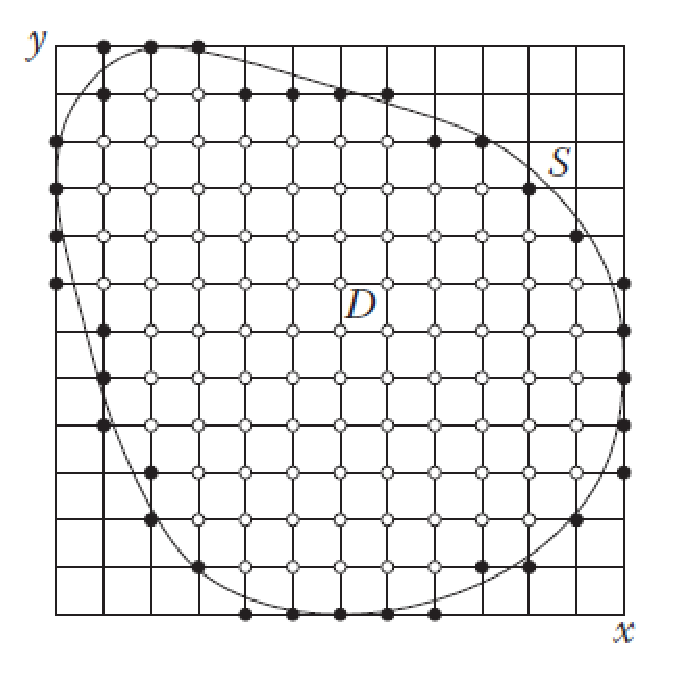
\includegraphics[scale=0.5]{Imagenes/condicionesEDP_01.eps}
	\caption{Malla/rejilla para implementar la solución. Los puntos negros indican los valores de frontera, mientras que los puntos blancos, es donde debe de calcularse la solución.}
\end{figure}
\end{frame}
\begin{frame}
\captionsetup{font=scriptsize,labelfont=scriptsize}
\frametitle{Condiciones con valores iniciales}
\begin{figure}
	\centering
	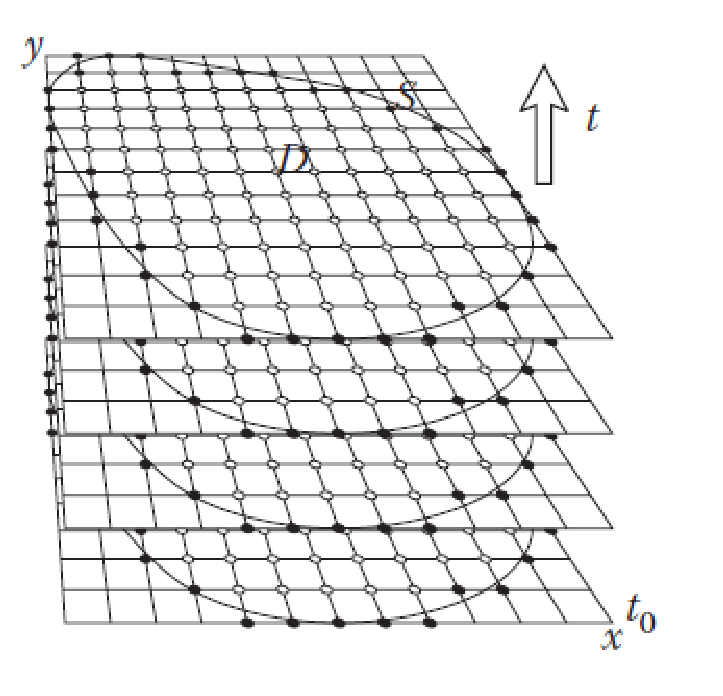
\includegraphics[scale=0.45]{Imagenes/condicionesEDP_02.eps}
	\caption{Se parte de un tiempo inicial $t_{0}$ y evoluciona en el tiempo $t$. Los puntos negros indican los valores de frontera, mientras que los puntos blancos, es donde debe de calcularse la solución.}
\end{figure}
\end{frame}
}
\begin{frame}
\frametitle{Solución a los problemas}
Aunque el objetivo principal de ambos tipos de problemas es el cálculo de la solución en una red espacial, la solución de estado estacionario para problemas con CDF se determina mediante un proceso numérico que converge simultáneamente en todo el dominio $D$.
\end{frame}
\begin{frame}
\frametitle{Solución a los problemas}
Mientras que en el caso de valores iniciales, la solución de todos los puntos en el dominio espacial, se propagan de manera recursiva en el tiempo, iniciando la solución a partir del instante $t_{0}$.
\end{frame}
\section{Solución de EDP Elípticas}
\frame[allowframebreaks]{\tableofcontents[currentsection, hideothersubsections]}
\subsection{CDF para EDP Elípticas}
\begin{frame}
\frametitle{Problemas CDF para EDP Elípticas}
Para revisar el proceso de discretización para problemas de CDF, consideremos la ecuación 2D de la ecuación de Poisson:
\begin{align}
\laplacian{u(x, y)} = \pdv[2]{u}{x} + \pdv[2]{u}{y} = f(x, y)
\label{eq:ecuacion_13_01}
\end{align}
\end{frame}
\begin{frame}
\frametitle{Problemas CDF para EDP Elípticas}
Escogemos un dominio rectangular de integración
\begin{align*}
D = [x_{\mbox{min}}, x_{\mbox{max}} ] \cp [y_{\mbox{min}}, y_{\mbox{max}} ]
\end{align*}
y se establecen las condiciones de frontera mixtas
\begin{align}
\left[ \alpha \: u + \beta \: \pdv{u}{n} \right]_{(x, y) \in S} = \gamma
\label{eq:ecuacion_13_02}
\end{align}
donde $\alpha(x, y)$, $\beta(x, y)$ y $\gamma(x, y)$ son funciones definidas en el dominio $S$.
\end{frame}
\begin{frame}
\frametitle{Problemas CDF para EDP Elípticas}
En particular, tenemos
\setbeamercolor{item projected}{bg=red!70!black,fg=white}
\setbeamertemplate{enumerate items}[circle]
\begin{enumerate}[<+->]
\item \emph{condiciones de Dirichlet} para $\beta = 0$ (valores de solución fijos)
\item \emph{condiciones de Neumann} para $\alpha = 0$ (derivadas normales fijas)
\item \emph{condiciones uniformes} para $\gamma = 0$
\end{enumerate}
\end{frame}
\subsection{Uso de diferencias finitas}
\begin{frame}
\frametitle{Uso de diferencias finitas}
Siguiendo la aproximación por el método de diferencias finitas, acotamos la solución para los valores $N_{x} \times N_{y}$ tal que $u_{ij} = u(x_{i}, y_{j})$ en los nodos de la malla espacial definida por
\begin{align*}
x_{i} = x_{\text{min}} + (i - 1) \: h_{x}, \hspace{0.5cm} i = 1, 2, \ldots, N_{x} \\
y_{i} = y_{\text{min}} + (j - 1) \: h_{y}, \hspace{0.5cm} j = 1, 2, \ldots, N_{y}
\end{align*}
\\
\bigskip
\pause
donde $h_{x}$ y $h_{y}$ corresponde al espaciamiento en la malla en las dos direcciones, como se aprecia en la siguiente figura:
\end{frame}
{\setbeamercolor{background canvas}{bg=white}
\begin{frame}
\frametitle{Malla para la solución}
\captionsetup{font=small,labelfont=small}
\begin{figure}
	\centering
	\includestandalone[scale=0.75]{Figuras/mallaSolucionEDP_01}
	\caption{Discretización de la malla para resolver la EDP.}
	\label{fig:figura_01}
\end{figure}
\end{frame}
}
\begin{frame}
\frametitle{Uso de diferencias finitas}
Similarmente a las técnicas de diferencias finitas que se vio en el Tema 3, nos aproximamos al operador laplaciano $\laplacian$ partiendo de la serie de Taylor de la solución en los puntos interiores del dominio $D$.
\\
\bigskip
En particular, a lo largo de la dirección $x$ tenemos, respectivamente, las diferencias hacia atrás y hacia delante:
\end{frame}
\begin{frame}
\frametitle{Uso de diferencias finitas}
Diferencias hacia atrás y hacia adelante
\fontsize{12}{12}\selectfont
\begin{align*}
u_{i-1, j} &= u_{i, j} - \dfrac{h_{x}}{1!} \left( \pdv{u}{x} \right)_{i, j} + \dfrac{h_{x}^{2}}{2!} \left( \pdv[2]{u}{x} \right)_{i, j} + \\
&- \dfrac{h_{x}^{3}}{3!} \left( \pdv[3]{u}{x} \right)_{i, j} + \order{h_{x}^{4}}  \\[1em]
u_{i+1, j} &= u_{i, j} + \dfrac{h_{x}}{1!} \left( \pdv{u}{x} \right)_{i, j} + \dfrac{h_{x}^{2}}{2!} \left( \pdv[2]{u}{x} \right)_{i, j} +\\
&+ \dfrac{h_{x}^{3}}{3!} \left( \pdv[3]{u}{x} \right)_{i, j} + \order{h_{x}^{4}}
\end{align*}
\end{frame}
\begin{frame}
\frametitle{Segunda derivada con diferencias finitas}
La expresión de diferencias finitas para la segunda derivada es
\begin{align}
\left( \pdv[2]{u}{x} \right)_{i,j} = \dfrac{u_{i+1, j} - 2 \: u_{i, j} + u_{i-1,j}}{h_{x}^{2}} + \order{h_{x}^{2}}
\label{eq:ecuacion_13_03}
\end{align}
\end{frame}
\begin{frame}
\frametitle{Segunda derivada con diferencias finitas}
El término del error $\order{h_{x}^{2}}$ se obtiene al cancelarse los términos de tercer orden en la expansión de $\order{h_{x}^{4}}$ y la correspondiente división entre $h_{x}^{2}$.
\\
\bigskip
Tenemos una fórmula de \emph{esquema de diferencias centrales}, ya que usa información de nodos distribuidos simétricamente sobre el punto donde se está evaluando la derivada.
\end{frame}
\begin{frame}
\frametitle{Segunda derivada con diferencias finitas}
De manera análoga, para la segunda derivada en la dirección $y$ es:
\begin{align}
\left( \pdv[2]{u}{y} \right)_{i,j} = \dfrac{u_{i, j+1} - 2 \: u_{i, j} + u_{i, j-1}}{h_{y}^{2}} + \order{h_{y}^{2}}
\label{eq:ecuacion_13_04}
\end{align}
\end{frame}
\begin{frame}
\frametitle{Uso de diferencias finitas}
Entonces, para el laplaciano de la función $u$ en el nodo $(x_{i}, y_{i})$, hay un esquema de diferencia en cinco puntos, que se correlaciona con la representación gráfica en la figura (\ref{fig:figura_01})
\end{frame}
\begin{frame}
\frametitle{El laplaciano de $u$}
\begin{align}
\begin{aligned}
\laplacian{u (x, y)}\eval_{i,j} &= \dfrac{1}{h_{y}^{2}} \: u_{i, j-1} + \dfrac{1}{h_{x}^{2}} \: u_{i-1, j} + \\[0.5em]
&- 2 \: \left( \dfrac{1}{h_{x}^{2}} + \dfrac{1}{h_{y}^{2}} \right) \: u_{i, j}  + \dfrac{1}{h_{x}^{2}} \: u_{i+1, j}  + \\[0.5em]
&+ \dfrac{1}{h_{y}^{2}} \: u_{i, j+1} + \order{h_{x}^{2} + h_{y}^{2}}
\end{aligned}
\label{eq:ecuacion_13_05}
\end{align}
\end{frame}
\begin{frame}
\frametitle{Uso de diferencias finitas}
Con ello se obtiene la siguiente expresión de diferencias finitas de la ecuación de Poisson en los puntos interiores del dominio $D$:
\begin{align}
\begin{aligned}
\dfrac{1}{h_{y}^{2}} \: u_{i, j-1} &+ \dfrac{1}{h_{x}^{2}} \: u_{i-1, j} - 2 \: \left( \dfrac{1}{h_{x}^{2}} + \dfrac{1}{h_{y}^{2}} \right) \: u_{i, j} + \\[0.5em]
&+ \dfrac{1}{h_{x}^{2}} \: u_{i+1, j} + \dfrac{1}{h_{y}^{2}} \: u_{i, j+1} = f_{i, j} \\[0.5em]
i &= 2, \ldots, N_{x-1}, \hspace{0.7cm} j = 2, \ldots, N_{y-1}
\end{aligned}
\label{eq:ecuacion_13_06}
\end{align}
donde $f_{i, j} \equiv f(x_{i}, y_{j})$.
\end{frame}
\subsection{Discretización del problema}
\begin{frame}
\frametitle{Discretización del problema}
El sistema lineal (\ref{eq:ecuacion_13_06}), teniendo como incógnitas los valores de la solución $u_{i, j}$ en los nodos de la malla, no contiene realmente suficientes ecuaciones para que la solución sea completamente determinada. 
\end{frame}
\begin{frame}
\frametitle{Discretización del problema}
Por otra parte, el esquema de discretización de cinco puntos empleado para el laplaciano impide la incorporación directa de las condiciones de frontera, que han de ser tratadas por separado.
\end{frame}
\begin{frame}
\frametitle{Discretización del problema}
Muy a menudo, el proceso de discretización de las condiciones de frontera es más intrincado que la discretización de las EDP mismas.
\\
\bigskip
En aras de la claridad, utilizamos en lo siguiente las aproximaciones de orden inferior para las condiciones de frontera mixtas.
\end{frame}
\begin{frame}
\frametitle{Discretización del problema}
Concretamente, considerando que las derivadas normales son positivas si están orientadas hacia fuera desde el dominio $D$, las condiciones límite a la izquierda y a la derecha ($i = 1$ e $i = N_{x}$) pueden expresarse como:
\end{frame}
\begin{frame}
\frametitle{Discretización del problema}
\begin{align*}
\alpha_{j}^{x_{\text{\tiny{min}}}} \: u_{1, j} &+ \beta_{j}^{x_{\text{\tiny{min}}}} \: \dfrac{u_{1, j} - u_{2, j}}{h_{x}} = \gamma_{j}^{x_{\text{\tiny{min}}}} \hspace{1cm} i = 1 \\[0.5em]
\alpha_{j}^{x_{\mbox{\tiny{max}}}} \: u_{N_{x}, j} &+ \beta_{j}^{x_{\text{\tiny{max}}}} \: \dfrac{u_{N_{x}, j} - u_{N_{x-1}, j}}{h_{x}} = \gamma_{j}^{x_{\text{\tiny{max}}}} \hspace{0.75cm} i = N_{x} \\[0.5em]
&j = 1, \ldots, N_{y}
\end{align*}
\end{frame}
\begin{frame}
\frametitle{Discretización del problema}
De manera similar, las condiciones de discretización para la frontera inferior y superior ($j = 1$ y $N_{y}$)
\begin{align*}
\alpha_{i}^{y_{\text{\tiny{min}}}} \: u_{i, 1} &+ \beta_{i}^{y_{\text{\tiny{min}}}} \: \dfrac{u_{i, 1} - u_{i, 2}}{h_{y}} = \gamma_{i}^{x_{\text{\tiny{min}}}} \hspace{0.75cm} j = 1 \\[0.5em]
\alpha_{i}^{y_{\text{\tiny{max}}}} \: u_{i, N} &+ \beta_{i}^{y_{\text{\tiny{max}}}} \: \dfrac{u_{i, N_{y}} - u_{i, N_{y-1}}}{h_{y}} = \gamma_{i}^{y_{\text{\tiny{max}}}} \hspace{0.75cm} j = N_{y} \\[0.5em]
&i = 1, \ldots, N_{x}
\end{align*}
\end{frame}
\begin{frame}
\frametitle{Simplificación en la notación}
Para simplificar las ecuaciones discretizadas y las CDF, definimos las siguientes cantidades
\begin{align}
k_{x} = \dfrac{1}{h_{x}^{2}}, \hspace{0.5cm} k_{y} = \dfrac{1}{h_{y}^{2}}, \hspace{0.5cm} k_{xy} = 2 \: \left( \dfrac{1}{h_{x}^{2}} + \dfrac{1}{h_{y}^{2}} \right)
\label{eq:ecuacion_13_07}
\end{align}
\end{frame}
\begin{frame}
\frametitle{Simplificación de las CDF}
Los coeficientes de frontera quedan:
\begin{align}
\begin{aligned}
\bar{\beta}_{i}^{y {\text{\tiny{min}}}} &= \beta_{i}^{y {\text{\tiny{min}}}} / \left( \alpha_{i}^{y {\text{\tiny{min}}}} \: h_{y}  + \beta_{i}^{y{\mbox{\tiny{min}}}} \right), \\[0.5em]
\bar{\beta}_{i}^{y {\text{\tiny{max}}}} &= \beta_{i}^{y {\text{\tiny{max}}}} / \left( \alpha_{i}^{y {\text{\tiny{max}}}} \: h_{y}  + \beta_{i}^{y{\mbox{\tiny{max}}}} \right), \\[0.5em]
\bar{\beta}_{j}^{x {\text{\tiny{min}}}} &= \beta_{x}^{x {\text{\tiny{min}}}} / \left( \alpha_{j}^{x {\text{\tiny{min}}}} \: h_{x}  + \beta_{j}^{x {\mbox{\tiny{min}}}} \right), \\[0.5em]
\bar{\beta}_{j}^{x {\text{\tiny{max}}}} &= \beta_{j}^{x {\text{\tiny{max}}}} / \left( \alpha_{j}^{x {\text{\tiny{max}}}} \: h_{x}  + \beta_{j}^{x {\mbox{\tiny{max}}}} \right)
\end{aligned}
\label{eq:ecuacion_13_08a}
\end{align}
\end{frame}
% \begin{frame}
% \frametitle{Simplificación de las CDF}
% Los coeficientes de frontera quedan:
% \begin{equation}
% \begin{aligned}
% \bar{\gamma}_{i}^{y {\text{\tiny{min}}}} &= \gamma_{i}^{y {\text{\tiny{min}}}} / \left( \alpha_{i}^{y {\text{\tiny{min}}}} + \beta_{i}^{y{\text{\tiny{min}}}} / h_{y} \right), \\
% \bar{\gamma}_{i}^{y {\text{\tiny{max}}}} &= \gamma_{i}^{y {\text{\tiny{max}}}} / \left( \alpha_{i}^{y {\text{\tiny{max}}}} + \beta_{i}^{y{\text{\tiny{max}}}} / h_{y} \right), \\
% \bar{\gamma}_{j}^{x {\text{\tiny{min}}}} &= \gamma_{j}^{x {\text{\tiny{min}}}} / \left( \alpha_{j}^{x {\text{\tiny{min}}}} + \beta_{j}^{x {\text{\tiny{min}}}} / h_{x} \right), \\
% \bar{\gamma}_{j}^{x {\text{\tiny{max}}}} &= \gamma_{j}^{x {\text{\tiny{max}}}} / \left( \alpha_{j}^{x {\text{\tiny{max}}}} + \beta_{j}^{x {\text{\tiny{max}}}} / h_{x} \right)
% \end{aligned}
% \label{eq:ecuacion_13_08b}
% \end{equation}
% \end{frame}
\begin{frame}
\frametitle{Sistema completo discretizado}
Con esto, el sistema lineal completo resultante de la discretización de la ecuación de Poisson y las condiciones de frontera mixtas adjuntas toma la siguiente forma:
\end{frame}
\begin{frame}
\frametitle{Sistema completo 1/3}
Para la frontera inferior
\begin{align}
u_{i, 1} - \bar{\beta}_{i}^{y {\text{\tiny{min}}}} \: u_{i, 2} = \bar{\gamma}_{i}^{y {\text{\tiny{min}}}}, \hspace{0.5cm} i = 1, \ldots, N_{x}, \hspace{0.3cm} j = 1
\label{eq:ecuacion_13_09}
\end{align}
\pause
Para la frontera izquierda
\begin{align}
u_{i, j} - \bar{\beta}_{i}^{y {\text{\tiny{min}}}} \: u_{2, j} = \bar{\gamma}_{i}^{y {\text{\tiny{min}}}}, \hspace{0.5cm} i = 1, \hspace{0.3cm} j = 2, \ldots, N_{y} - 1
\label{eq:ecuacion_13_10}
\end{align}
\end{frame}
\begin{frame}
\frametitle{Sistema completo 2/3}
Para los puntos interiores
\begin{align}
\begin{aligned}
k_{y} \: u_{i, j-1} &+ k_{x} \: u_{i-1, j} - k_{xy} \: u_{i, j} + k_{x} \: u_{i+1, j} + \\
&+ k_{y} \: u_{i, j+1} =  f_{i,j} \\
i &= 2, \ldots, N_{x} - 1, \hspace{1cm} j = 2, \ldots, N_{y} - 1 \hspace{2cm}
\end{aligned}
\label{eq:ecuacion_13_11}
\end{align}
\end{frame}
\begin{frame}
\frametitle{Sistema completo 3/3}
Para la frontera derecha
\begin{align}
- \bar{\beta}_{j}^{x {\text{\tiny{max}}}} \:  u^{}_{N_{x-1}, j} &+ u^{}_{N_{x},j}  =  \bar{\gamma}_{j}^{x {\text{\tiny{max}}}} \\[0.5em]
&i = N_{x}, \hspace{0.3cm} j = 2, \ldots, N_{y} - 1
\label{eq:ecuacion_13_12}
\end{align}
\pause
Para la frontera superior
\begin{align}
- \bar{\beta}_{j}^{y {\text{\tiny{max}}}} \: u^{}_{i, N_{y-1}} &+ u^{}_{i, N_{y}}  =  \bar{\gamma}_{i}^{y {\text{\tiny{max}}}} \\[0.5em]
&i = 1, \ldots, N_{x}, \hspace{0.3cm} j = N_{y}
\label{eq:ecuacion_13_13}
\end{align}
\end{frame}
\begin{frame}
\frametitle{Re-escribiendo el sistema}
El sistema discretizado completo se puede re-escribir de una forma general, lo que ayuda a revelar su estructura:
\begin{align}
\begin{aligned}
a_{i}^{j} \: u_{i, j-1} &+ b_{ai}^{j} \: u_{i-1, j} + b_{bi}^{j} \: u_{i, j} + \\[0.5em]
&+ b_{ci}^{j} \: u_{i+1, j} + c_{i}^{j} \: u_{i, j+1} = d_{i}^{j} \\[0.5em]
&i = 1, \ldots, N_{x}, \hspace{0.5cm} j = 1, \ldots, N_{y}
\end{aligned}
\label{eq:ecuacion_13_14}
\end{align}
\end{frame}
\begin{frame}
\frametitle{Re-escribiendo el sistema}
Teniendo en cuenta que la ecuación discretizada centrada alrededor del nodo malla $(i, j)$ no solo conecta los cinco valores vecinos $(u_{i, j-1}, u_{i-1, j}, u_{i,j}, u_{i+1, j}, u_{i, j+1})$, sino todos los valores en los tres renglones contiguos $j-1, j, j+1$.
\end{frame}
\begin{frame}
\frametitle{Re-escribiendo el sistema}
 El sistema puede expresarse como
\begin{align}
\begin{aligned}
\sum_{i^{\prime} = 1}^{N_{x}} &\left[ A_{ii^{\prime}}^{j} \: u_{i^{\prime}, j-1} + B_{ii^{\prime}}^{j} \: u_{i^{\prime}, j} + C_{ii^{\prime}}^{j} \: u_{i^{\prime}, j+1}  \right] = d_{i}^{j} \\[0.5em]
&i = 1, \ldots, N_{x} \hspace{0.5cm} j = 1, \ldots, N_{y}
\end{aligned}
\label{eq:ecuacion_13_15}
\end{align}
\end{frame}
\begin{frame}
\frametitle{Re-escribiendo el sistema}
Donde los bloques $N_{x} \times N_{x}$ de
\begin{align*}
\mathbf{A}^{j} &= [A_{ii^{\prime}}^{j}]_{N_{x} N_{x}} \\[0.5em]
\mathbf{B}^{j} &= [B_{ii^{\prime}}^{j}]_{N_{x} N_{x}} \\[0.5em]
\mathbf{C}^{j} &= [C_{ii^{\prime}}^{j}]_{N_{x} N_{x}} \\
\end{align*}   
tienen los siguientes elementos:
\end{frame}
\begin{frame}
\frametitle{Re-escribiendo el sistema}
\begin{align}
\begin{aligned}
A_{ii^{\prime}}^{j} &= a_{i}^{j} \: \delta_{ii^{\prime}} \\[0.5em]
B_{ii^{\prime}}^{j} &= \begin{cases}
b_{ai}^{j} & \mbox{ si } i^{\prime} = i-1 \\[0.25em]
b_{bi}^{j} & \mbox{ si } i^{\prime} = i \\[0.25em]
b_{ci}^{j} & \mbox{ si } i^{\prime} = i+1 \\[0.25em]
0 & \mbox{ si } i^{\prime} \neq i, i \pm 1 \end{cases} \\[0.5em]
C_{ii^{\prime}}^{j} &= c_{i}^{j} \: \delta_{ii^{\prime}}
\end{aligned}
\label{eq:ecuacion:13_16}
\end{align}
\end{frame}
\subsection{Sistema matricial en banda}
\begin{frame}
\frametitle{Sistema matricial en banda}
Usando estos bloques, del sistema matricial completo se puede ver que forma un bloque trigiadonal y su estructura en banda es la siguiente:
\end{frame}
{\setbeamercolor{background canvas}{bg=white}
\begin{frame}
\frametitle{Sistema tridiagonal y en banda}
\begin{figure}
	\centering
	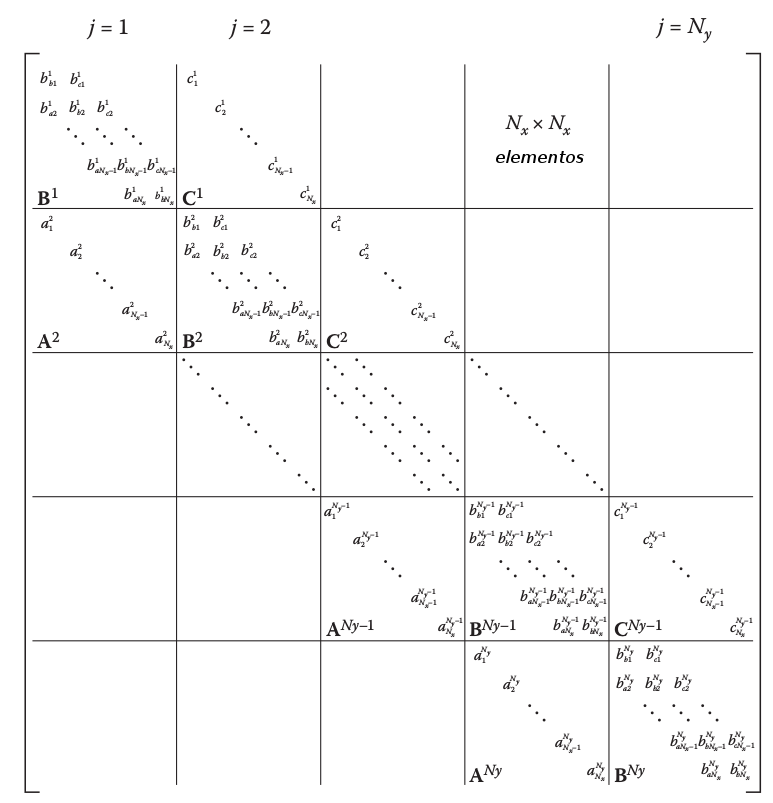
\includegraphics[scale=0.27]{Imagenes/Sistema_Matricial_Completo.png}
\end{figure}    
\end{frame}
}
\begin{frame}
\frametitle{Ajustado el sistema discretizado}
Al definir los vectores $\vb{u}^{j} = [u_{i^{\prime}, j}]_{N_{x}}$ y $\vb{d}^{j} = [d_{i}^{j}]_{N_{x}}$, con $\vb{u}^{j}$ teniendo como componentes los valores de solución $N_{x}$ en la fila $j$ y $\mathbf{d}^{j}$ que contienen los términos correspondientes del lado derecho, el sistema discretizado toma la forma:
\pause
\begin{align}
\vb{A}^{j} \: \vb{u}^{j-1} &+ \vb{B}^{j} \: \vb{u}^{j+1} +  \vb{C}^{j} \: \vb{u}^{j+1} = \vb{d}^{j}, \\[0.5em]
&j = 1, 2, \ldots, N_{y}
\label{eq:ecuacion_13_17}
\end{align}
\end{frame}
\begin{frame}
\frametitle{Ajustando el sistema discretizado}
Vemos un conjunto de ecuaciones matriciales conectando los vectores $\vb{u}^{j-1}$, $\vb{u}^{j}$ y $\vb{u}^{j+1}$, que son, las soluciones de los renglones $j-1$, $j$ y $j+1$, respectivamente.
\end{frame}
\begin{frame}
\frametitle{Ajustando el sistema discretizado}
En notación matricial, la estructura en bloques tridiagonal puede leerse como:
\pause
\fontsize{10}{10}\selectfont
\begin{align}
\begin{bmatrix}
\mathbf{B^{1}} & \mathbf{C^{1}} & & & \\
\mathbf{A^{2}} & \mathbf{B^{2}} & \mathbf{C^{2}} & & \\
 & \ddots & \ddots & \ddots & \\
 & & \mathbf{A^{N_{y}}-1} & \mathbf{B^{N_{y}}-1} & \mathbf{C^{N_{y}}-1}& \\
 & & & \mathbf{A}^{N_{y}} & \mathbf{B}^{N_{y}} 
\end{bmatrix}
\begin{bmatrix}
\mathbf{u}^{1} \\
\mathbf{u}^{2} \\
\vdots \\
\mathbf{u}^{N_{y} - 1} \\
\mathbf{u}^{N_{y}}
\end{bmatrix} = 
\begin{bmatrix}
\mathbf{d}^{1} \\
\mathbf{d}^{2} \\
\vdots \\
\mathbf{d}^{N_{y} - 1} \\
\mathbf{d}^{N_{y}}
\end{bmatrix}
\label{eq:ecuacion_13_18}
\end{align}
\end{frame}
\subsection{Solución al sistema completo}
\begin{frame}
\frametitle{Solución del sistema completo}
El sistema (\ref{eq:ecuacion_13_18}) puede resolverse, en principio, usando los dos tipos de métodos que consideran la estructura escasa de la matriz:
\setbeamercolor{item projected}{bg=red!70!black,fg=white}
\setbeamertemplate{enumerate items}[circle]
\begin{enumerate}[<+->]
\item \emph{Métodos directos: } que utilizan la inversión recursiva de los bloques que componen a la matriz.
\item \emph{Métodos indirectos: } como el de Jacobi o Gauss-Seidel y de sobrerrelajación.
\end{enumerate}
\end{frame}
\begin{frame}
\frametitle{Estrategia de solución}
Debido a la implementación menos elaborada y al escalamiento más favorable de los cálculos con el tamaño del sistema, para problemas con más de dos dimensiones o con límites de dominio complejos, los métodos iterativos resultan ser preferibles para resolver el sistema lineal obtenido al discretizar la EDP con CDF.
\end{frame}
\begin{frame}
\frametitle{Estrategia de solución}
Por lo tanto, limitamos la siguiente discusión al método iterativo de \emph{Gauss-Seidel}, que muestra en la práctica un espectro más amplio de aplicaciones, que también es adecuado para resolver problemas de valores propios para EDP.
\end{frame}
\begin{frame}
\frametitle{Solución}
Podemos re-escribir el sistema con la siguiente forma general
\begin{align}
\vb{A \cdot u} =  \vb{d}
\label{eq:ecuacion_13_19} 
\end{align}
\pause
Y considerar la descomposición:
\begin{align}
\vb{A} = \vb{L} + \vb{D} + \vb{U}
\label{eq:ecuacion_13_20}
\end{align}
donde: $\mathbf{L}$ es una matriz triangular inferior, $\mathbf{D}$ es una matriz diagonal, $\mathbf{U}$ es una matriz triangular superior.
\end{frame}
\begin{frame}
\frametitle{solución}
En el \emph{Método de Jacobi}, los elementos de la diagonal se expresan y la solución se itera de acuerdo a la relación:
\begin{align*}
\vb{D} \cdot \vb{u}^{(r)} = \vb{d} - (\vb{L} + \vb{U}) \cdot \vb{u}^{(r-1)}
\end{align*}
\pause
o equivalentemente
\begin{align}
\vb{u}^{(r)} = \vb{D}^{-1} \cdot \left[ \vb{d} - (\vb{L} + \vb{U}) \cdot \vb{u}^{(r-1)} \right]
\label{eq:ecuacion_13_21}
\end{align}
donde $r = 1, 2, \ldots$ es el orden de la aproximación a la solución.
\end{frame}
\begin{frame}
\frametitle{Solución}
Como $\vb{D}$ es diagonal, la inversa $\vb{D}^{-1}$ también es diagonal y contiene simplemente las inversas de los elementos diagonales de $\vb{D}$.
\\
\bigskip
El método de Jacobi converge para las matrices que son diagonalmente dominantes y esta condición generalmente se satisface en el marco de las metodologías de diferencias finitas.
\end{frame}
\begin{frame}
\frametitle{Solución}
Refiriéndose específicamente a la ecuación (\ref{eq:ecuacion_13_11} para los puntos de malla interior de los sistemas discretizados (\ref{eq:ecuacion_13_09}) - (\ref{eq:ecuacion_13_13}), los componentes de solución diagonal son los que están situados en el centro de los esquemas de discretización tipo estrella, es decir, $u_{i,j}$.
\end{frame}
\begin{frame}
\frametitle{Solución}
Correspondientemente, la solución se itera en función de la relación de recurrencia:
\begin{align}
\begin{aligned}
u_{i,j}^{(r)} &= \left[ k_{x} \: \left( u_{i-1,j}^{(r-1)} + u_{i+1, j}^{(r-1)} \right) + \right. \\
&+ \left. k_{y} \: \left( u_{i,j-1}^{(r-1)} + u_{i, j+1}^{(r-1)} \right) - f_{i,j} \right] / k_{xy}
\end{aligned}
\label{eq:ecuacion_13_22} 	
\end{align}
\pause
Está definiendo para el método de Jacobi, que todos los valores de solución empleados en el lado derecho provienen de la iteración anterior: $(r - 1)$.
\end{frame}
\begin{frame}
\frametitle{Solución}
Suponiendo que el algoritmo se ejecuta dentro de los bucles anidados, en orden creciente de los índices $i$ y $j$ al calcular $u_{i,j}^{(r)}$, los componentes actualizados de $u_{i, j-1}^{(r)}$ y $u_{i-1, j}^{(r)}$ ya están disponibles.
\end{frame}
\subsection{El método de Gauss-Seidel}
\begin{frame}
\frametitle{Solución}
Su uso inmediato es específico en el \emph{método de Gauss-Seidel} y la correspondiente relación de recurrencia formal toma la forma:
\begin{align}
\begin{aligned}
u_{i,j}^{(r)} &= \left[ k_{x} \: \left( u_{i-1,j}^{(r)} + u_{i+1, j}^{(r-1)} \right) + \right. \\
&+ \left. k_{y} \: \left( u_{i,j-1}^{(r)} + u_{i, j+1}^{(r-1)} \right) - f_{i,j} \right] / k_{xy}
\end{aligned}
\label{eq:ecuacion_13_23} 	
\end{align}
\end{frame}
\begin{frame}
\frametitle{Solución}
Por lo tanto, a diferencia del método de Jacobi, $u_{i,j}^{(r)}$ es calculado usando los más recientes componentes de $u_{i,j-1}^{(r)}$ y $u_{i-1, j}^{(r)}$, y no de sus predecesores $u_{i,j-1}^{(r-1)}$ y $u_{i-1, j}^{(r-1)}$.
\end{frame}
\begin{frame}
\frametitle{Solución}
Además de la velocidad de convergencia mejorada, el método de Gauss-Seidel también requiere una sola matriz (no dos) para almacenar la solución.
\\
\bigskip
Este arreglo puede contener al mismo tiempo componentes de ambas aproximaciones $\vb{u}^{(r-1)}$ y $\vb{u}^{(r)}$, que se actualizan continuamente y se pueden utilizar inmediatamente después de su cálculo.
\end{frame}
\begin{frame}
\frametitle{Ecuaciones obtenidas con Gauss-Seidel}
Las ecuaciones que describen la solución iterativa del sistema discretizado (\ref{eq:ecuacion_13_09}) -  (\ref{eq:ecuacion_13_13}) con condiciones de frontera mixtas, basadas en el método de Gauss-Seidel, ahora se pueden compilar de la siguiente manera:
\end{frame}
\begin{frame}
\frametitle{Ecuaciones obtenidas con Gauss-Seidel 1/3}
Para la frontera inferior
\begin{align}
\begin{aligned}
u_{i, 1}^{(r)} = \bar{\beta}_{i}^{y {\text{\tiny{min}}}} \: &u_{1,2}^{(r-1)} + \bar{\gamma}_{i}^{y {\text{\tiny{min}}}}, \\[0.5em]
&i = 1, \ldots, N_{x}, \hspace{0.3cm} j = 1
\end{aligned}
\label{eq:ecuacion_13_24}
\end{align}
\pause
Para la frontera izquierda
\begin{align}
\begin{aligned}
u_{i, j}^{(r)} = \bar{\beta}_{i}^{x {\text{\tiny{min}}}} \: &u_{2, j}^{(r-1)} + \bar{\gamma}_{j}^{x {\text{\tiny{min}}}}, \hspace{0.5cm} i = 1, \\[0.5em]
&j = 2, \ldots, N_{y} - 1
\end{aligned}
\label{eq:ecuacion_13_25}
\end{align}
\end{frame}
\begin{frame}
\frametitle{Ecuaciones obtenidas con Gauss-Seidel 2/3}
Para los puntos interiores
\begin{equation}
\begin{aligned}
u_{i,j}^{(r)} &= \left[ k_{x} \left( u_{i, j-1}^{(r)} u_{i+1, j}^{(r-1)} \right) + \right. \\[0.5em]
&+ \left. k_{y} \left( u_{i, j-1}^{(r)} + u_{i, j+1}^{(r-1)} \right) - f_{i,j} \right] / k_{xy} \\[0.5em]
i &= 2, \ldots, N_{x} - 1, \hspace{1cm} j = 2, \ldots, N_{y} - 1 \hspace{2cm}
\end{aligned}
\label{eq:ecuacion_13_26}
\end{equation}    
\end{frame}
\begin{frame}
\frametitle{Ecuaciones obtenidas con Gauss-Seidel 3/3}
\frametitle{Sistema completo 3/3}
Para la frontera derecha
\begin{align}
\begin{aligned}
u_{N_{x},j}^{(r)} = \bar{\beta}_{j}^{x {\text{\tiny{max}}}} \: &u_{N_{x-1}, j}^{(r-1)} + \bar{\gamma}_{j}^{x {\text{\tiny{max}}}} \\[0.5em]
&i = N_{x}, \hspace{0.3cm} j = 2, \ldots, N_{y} - 1
\end{aligned}
\label{eq:ecuacion_13_27}
\end{align}
\pause
Para la frontera superior
\begin{align}
\begin{aligned}
u_{i, N_{y}}^{(r)} = \bar{\beta}_{j}^{y {\text{\tiny{max}}}} \: &u_{N_{x-1}, j}^{(r-1)} + \bar{\gamma}_{i}^{y {\text{\tiny{max}}}} \\[0.5em]
&i = 1, \ldots, N_{x}, \hspace{0.3cm} j = N_{y}
\end{aligned}
\label{eq:ecuacion_13_28}
\end{align}
\end{frame}
\begin{frame}
\frametitle{Punto de paro}
El proceso recursivo (\ref{eq:ecuacion_13_24}) - (\ref{eq:ecuacion_13_28}) continua, en principio, hasta que la \emph{diferencia máxima relativa} entre los componentes de la solución de dos iteraciones consecutivas son menores a una tolerencia definida $\varepsilon$:     
\begin{align}
\max_{i,j} \abs{1 - u_{ij}^{(r-1)} / u_{ij}^{(r)}} \leq \varepsilon
\label{eq:ecuacion_13_29}
\end{align}
\end{frame}
\begin{frame}
\frametitle{Punto de paro}
Para los componentes que se anulan, este criterio de convergencia debería emplear la diferencia \emph{absoluta} máxima:
\begin{align*}
\max_{i,j} \abs{u_{ij}^{(r)} / u_{ij}^{(r-1)}}
\end{align*}
\end{frame}
\subsection{Algoritmos con \texttt{python}}
\begin{frame}
\frametitle{Dos algoritmos con \python}
Las rutinas \funcionazul{PoissonCero} y \funcionazul{PoissonXY} que se muestran a continuación, son implementaciones cada vez más complejas que nos servirán para resolver el sistema lineal ecs. (\ref{eq:ecuacion_13_24}) - (\ref{eq:ecuacion_13_28}), para la ecuación de Poisson discretizada mediante el método de Gauss-Seidel.
\end{frame}
\subsection*{La función \texttt{PoissonCero}}
\begin{frame}
\frametitle{La función \texttt{PoissonCero}}
Resuelve la ecuación de Poisson en 2D en coordenadas cartesianas con condiciones de tipo Dirichlet en una malla regular $(nx \cp ny)$ con nodos (\funcionazul{x[], y[]}) utilizando el método de Gauss-Seidel.
\\
\bigskip
La solución \funcionazul{u[][]} converge con precisión relativa \funcionazul{eps}. Se devuelve una bandera de error: $0$- ejecución normal. Utiliza: \funcionazul{Func (x, y)} y el lado derecho (\funcionazul{RHS}) de la ecuación de Poisson.
\end{frame}
\begin{frame}[allowframebreaks, plain, fragile]
\frametitle{Función \texttt{PoissonCero}}
\begin{lstlisting}[caption=Código para la función \texttt{PoissonCero}, style=FormattedNumber, basicstyle=\linespread{1.1}\ttfamily=\small, columns=fullflexible]
def PoissonCero(u, x, y, nx, ny, eps, Func):
   itmax = 10000

   f = [[0]*(ny+1) for i in range(nx+1)]

   hx = (x[nx]-x[1])/(nx-1); kx = 1e0/(hx*hx)
   hy = (y[ny]-y[1])/(ny-1); ky = 1e0/(hy*hy) 
   kxy = 2e0*(kx + ky)

   for j in range(2, ny):
      for i in range(2, nx): f[i][j] = Func(x[i], y[j])

   for it in range(1, itmax+1):
      err = 0e0
      for j in range(2, ny):
         for i in range(2, nx):
            uij = (kx*(u[i-1][j] + u[i+1][j]) +
                   ky*(u[i][j-1] + u[i][j+1]) - f[i][j]) / kxy
            eij = 1e0 - u[i][j]/uij if uij else uij - u[i][j]
            if (fabs(eij) > err): err = fabs(eij)
            u[i][j] = uij

      if (err <= eps): break

   if (it >= itmax):
      print("PoissonCero: Se excedio el numero maximo de iteraciones!"); return 1
   return 0
\end{lstlisting}
\end{frame}
\subsection*{La función \texttt{PoissonXY}}
\begin{frame}
\frametitle{La función \texttt{PoissonXY}}
Resuelve la ecuación de Poisson en 2D en coordenadas cartesianas en una malla regular ($nx \cp ny$) con nodos \funcionazul{(x [], y [])} utilizando el método de Gauss-Seidel.
\\
\bigskip
La solución \funcionazul{u [] []} converge con precisión relativa \funcionazul{eps}. Se devuelve una bandera de error: $0$ - ejecución normal.
\end{frame}
\begin{frame}
\frametitle{La función \texttt{PoissonXY}}
Llamadas: \funcionazul{Func (x, y)} y el lado derecho de la ecuación de Poisson \funcionazul{RHS}.
\\
\bigskip
Ccondiciones de frontera: \\
\funcionazul{CondX (y, alf\_min, bet\_min, gam\_min, alf\_max, bet\_max, gam\_max)}
\\
\medskip
\funcionazul{CondY (x, alf\_min, bet\_min, gam\_min, alf\_max, bet\_max, gam\_max)}
\end{frame}
\begin{frame}[allowframebreaks, fragile, plain]
\frametitle{Código para \texttt{PoissonXY}}
\begin{lstlisting}[caption=Código para la función \texttt{PoissonXY}, style=FormattedNumber, basicstyle=\linespread{1.1}\ttfamily=\small, columns=fullflexible]
def PoissonXY(u, x, y, nx, ny, eps, Func, CondX, CondY):
    itmax = 10000
 
    f = [[0]*(ny+1) for i in range(nx+1)]
    betXmin = [0]*(ny+1); betXmax = [0]*(ny+1)
    gamXmin = [0]*(ny+1); gamXmax = [0]*(ny+1)
    betYmin = [0]*(nx+1); betYmax = [0]*(nx+1)
    gamYmin = [0]*(nx+1); gamYmax = [0]*(nx+1)
 
    hx = (x[nx]-x[1])/(nx-1); kx = 1e0/(hx*hx)
    hy = (y[ny]-y[1])/(ny-1); ky = 1e0/(hy*hy) 
    kxy = 2e0*(kx + ky)
 
    for j in range(2,ny):
       for i in range(2,nx): f[i][j] = Func(x[i],y[j])
                                                         
    for i in range(1,nx+1):
       (alf_\textunderscore_min,bet_\textunderscore_min,gam_\textunderscore_min,alf_\textunderscore_max,bet_\textunderscore_max,gam_\textunderscore_max) = CondY(x[i])
       betYmin[i] = bet_\textunderscore_min/(alf_\textunderscore_min*hy + bet_\textunderscore_min)
       gamYmin[i] = gam_\textunderscore_min/(alf_\textunderscore_min + bet_\textunderscore_min/hy)
       betYmax[i] = bet_\textunderscore_max/(alf_\textunderscore_max*hy + bet_\textunderscore_max)
       gamYmax[i] = gam_\textunderscore_max/(alf_\textunderscore_max + bet_\textunderscore_max/hy)
 
    for j in range(2,ny):
       (alf_\textunderscore_min,bet_\textunderscore_min,gam_\textunderscore_min,alf_\textunderscore_max,bet_\textunderscore_max,gam_\textunderscore_max) = CondX(y[j])
       betXmin[j] = bet_\textunderscore_min/(alf_\textunderscore_min*hx + bet_\textunderscore_min)
       gamXmin[j] = gam_\textunderscore_min/(alf_\textunderscore_min + bet_\textunderscore_min/hx)
       betXmax[j] = bet_\textunderscore_max/(alf_\textunderscore_max*hx + bet_\textunderscore_max)
       gamXmax[j] = gam_\textunderscore_max/(alf_\textunderscore_max + bet_\textunderscore_max/hx)
 
    for it in range(1,itmax+1): 
       err = 0e0
       j = 1
       for i in range(1,nx+1):
          uij = betYmin[i]*u[i][2] + gamYmin[i]
          eij = 1e0 - u[i][j]/uij if uij else uij - u[i][j]
          if (fabs(eij) > err): err = fabs(eij)
          u[i][j] = uij
 
       for j in range(2,ny):
          i = 1
          uij = betXmin[j]*u[i+1][j] + gamXmin[j]
          eij = 1e0 - u[i][j]/uij if uij else uij - u[i][j]
          if (fabs(eij) > err): err = fabs(eij)
          u[i][j] = uij
 
          for i in range(2,nx):
             uij = (kx*(u[i-1][j] + u[i+1][j]) +
                    ky*(u[i][j-1] + u[i][j+1]) - f[i][j]) / kxy
             eij = 1e0 - u[i][j]/uij if uij else uij - u[i][j] 
             if (fabs(eij) > err): err = fabs(eij)
             u[i][j] = uij
 
          i = nx
          uij = betXmax[j]*u[i-1][j] + gamXmax[j]
          eij = 1e0 - u[i][j]/uij if uij else uij - u[i][j]
          if (fabs(eij) > err): err = fabs(eij)
          u[i][j] = uij
 
       j = ny
       for i in range(1,nx+1):
          uij = betYmax[i]*u[i][ny-1] + gamYmax[i]
          eij = 1e0 - u[i][j]/uij if uij else uij - u[i][j]
          if (fabs(eij) > err): err = fabs(eij)
          u[i][j] = uij
 
       if (err <= eps): break
 
    if (it >= itmax):
       print("PoissonXY: Se excedio el numero maximo de iteraciones !"); return 1
    return 0
\end{lstlisting}
\end{frame}
\begin{frame}
\frametitle{Sobre los códigos}
La rutina \funcionazul{PoissonCero} está diseñada para operar solo con condiciones de contorno de Dirichlet.
\\
\bigskip
En consecuencia, de todo el sistema (\ref{eq:ecuacion_13_24}) - (\ref{eq:ecuacion_13_28}), solo necesita iterar la ecuación \ref{eq:ecuacion_13_26} para los puntos interiores del dominio.
\end{frame}
\begin{frame}
\frametitle{Sobre los códigos}
La rutina recibe la aproximación inicial de la solución, incluidos los valores límite, por medio de la matriz \funcionazul{u [] []}, que también devuelve la solución tras la ejecución.
\end{frame}
\begin{frame}
\frametitle{Sobre los códigos}
Las coordenadas cartesianas de los puntos de malla uniformemente espaciados se reciben a través de las matrices \funcionazul{x []} e \funcionazul{y []}, con los parámetros \funcionazul{nx} y \funcionazul{ny} pasando los números correspondientes de nodos, y \funcionazul{eps}, la tolerancia relativa que se aplicará a la solución.
\end{frame}
\begin{frame}
\frametitle{Sobre los códigos}
La rutina \funcionazul{PoissonXY} generaliza las funcionalidades de la rutina \funcionazul{PoissonCero}, pudiendo resolver problemas con condiciones de frontera mixtas, basándose en el conjunto completo de ecuaciones discretizadas (\ref{eq:ecuacion_13_24}) a (\ref{eq:ecuacion_13_28}).
\end{frame}
\begin{frame}
\frametitle{Sobre los códigos}
La lista de argumentos de los dos solucionadores de Poisson es similar, con la matriz \funcionazul{u [] []} pasando a la entrada una aproximación inicial y regresando a la salida la solución final.
\end{frame}
\begin{frame}
\frametitle{Sobre los códigos}
Los argumentos de procedimiento complementarios \funcionazul{Func}, \funcionazul{CondX} y \funcionazul{CondY} de \funcionazul{PoissonXY} proporcionan los nombres reales de las rutinas de usuario que devuelven los valores de la función del lado derecho $f(x, y)$ y, respectivamente, los coeficientes que definen las condiciones de contorno.
\end{frame}
\begin{frame}
\frametitle{Sobre los códigos}
Específicamente, para una \funcionazul{y} dada, se espera que la función \funcionazul{CondX} devuelva los coeficientes \funcionazul{alf\_min}, \funcionazul{bet\_min} y \funcionazul{gam\_min}, que definen las condiciones en la dirección $x$, normal al límite izquierdo, así como \funcionazul{alf\_max}, \funcionazul{bet\_max} y \funcionazul{gam\_max}, correspondientes hacia el límite derecho.
\end{frame}
\begin{frame}
\frametitle{Sobre los códigos}
De manera similar, para cada \funcionazul{x} dada, se espera que la función \funcionazul{CondY} devuelva los coeficientes que definen la solución en la dirección $y$ en los límites inferior y superior, respectivamente.
\end{frame}
\begin{frame}
\frametitle{Sobre los códigos}
En la primera fase, \funcionazul{PoissonXY} determina los coeficientes auxiliares $\bar{\beta}$ y $\bar{\gamma}$ de acuerdo con la ecuación \ref{eq:ecuacion_13_08a} y almacena los valores de la función del lado derecho $f (x, y)$.
\end{frame}
\begin{frame}
\frametitle{Sobre los códigos}
Una vez que se preparan las cantidades constantes, la rutina ingresa al bucle Gauss-Seidel, donde la solución se actualiza en cada iteración en secuencia en el límite inferior, en el límite izquierdo, en los puntos de malla interiores, en el límite derecho y, finalmente , en el límite superior.
\end{frame}
\begin{frame}
\frametitle{Sobre los códigos}
Junto con la solución actualizada, también se registra el error relativo máximo de los componentes de la solución, como estimación de error.
\\
\bigskip
El proceso de Gauss-Seidel continúa hasta que \funcionazul{err} cae por debajo de la tolerancia elegida \funcionazul{eps}.
\\
\bigskip
Si se excede el número máximo de iteraciones predefinido, se emite un mensaje de error y se devuelve una bandera de error distinto de cero.
\end{frame}
\subsection{Ejercicio de la Ec. de Poisson}
\begin{frame}
\frametitle{Ejercicio de la Ec. de Poisson}
Como ejercicio para el uso de la rutina \funcionazul{PoissonXY}, consideramos el problema asociado con la ecuación de Poisson:
\begin{align}
\pdv[2]{u}{x} + \pdv[2]{u}{y} = \cos(x + y) - \cos (x - y)
\label{eq:ecuacion_13_30}
\end{align}
que queremos resolver en el dominio:
\begin{align*}
\mathbb{D} = [- \pi, \pi] \cp [-\pi, \pi]
\end{align*}
\end{frame}
\begin{frame}
\frametitle{Condiciones de frontera}
Que está sujeto a las condiciones de frontera:
\begin{align}
\begin{aligned}
u(\pm \pi, y) &= 0, \hspace{1cm} y \in [-\pi, \pi] \\[0.5em]
u(x, \pm \pi) &= 0, \hspace{1cm} x \in [-\pi, \pi]
\end{aligned}
\label{eq:ecuacion_13_31}
\end{align}
\pause
La solución analítica es $u(, y)=\sin x \, \sin y$ (podrías demostrar como ejercicio moral), ésta solución la podremos utilizar como referencia.
\end{frame}
\begin{frame}
\frametitle{Código para resolver}
Se presenta el siguiente código con el cual resolveremos el problema planteado.sa
\\
\bigskip
Revisaremos previamente unas secciones del código para aclarar su funcionamiento.
\end{frame}
\begin{frame}
\frametitle{Operación del código}
Se definen las funciones \funcionazul{Func}, \funcionazul{CondX}, \funcionazul{CondY}, que devuelven respectivamente: los valores del lado derecho de la EDP, así como los coeficientes que definen las condiciones de contorno.
\end{frame}
\begin{frame}
\frametitle{Operación del código}
El código inicializa los arreglos \funcionazul{x[]} e \funcionazul{y[]} con la coordenadas de la malla de puntos e inicia el cálculo con una aproximación inicial trivial, en donde todos los componentes de la solución se dejan en $0$.
\end{frame}
\begin{frame}
\frametitle{Operación del código}
La solución que devuelve \funcionazul{PoissonXY} para una malla de $51 \cp 51$ puntos, con una tolerancia relativa de $\varepsilon = \num{d-5}$, se escribe en un archivo de salida, que posteriormente se utilizará para graficar la solución.
\end{frame}
\begin{frame}[allowframebreaks, fragile, plain]
\frametitle{Código completo}
\begin{lstlisting}[caption=Código para resolver la ec. de Poisson, style=FormattedNumber, basicstyle=\linespread{1.1}\ttfamily=\small, columns=fullflexible]
import numpy as np
from ModuloPoisson import PoissonXY

def Func(x, y):
   return np.cos(x+y) - np.cos(x-y)

def CondX(y):
   alf_\textunderscore_min = 1e0; bet_\textunderscore_min = 0e0; gam_\textunderscore_min = 0e0
   alf_\textunderscore_max = 1e0; bet_\textunderscore_max = 0e0; gam_\textunderscore_max = 0e0
   return (alf_\textunderscore_min, bet_\textunderscore_min, gam_\textunderscore_min, alf_\textunderscore_max, bet_\textunderscore_max, gam_\textunderscore_max)

def CondY(x):
   alf_\textunderscore_min = 1e0; bet_\textunderscore_min = 0e0; gam_\textunderscore_min = 0e0
   alf_\textunderscore_max = 1e0; bet_\textunderscore_max = 0e0; gam_\textunderscore_max = 0e0
   return (alf_\textunderscore_min, bet_\textunderscore_min, gam_\textunderscore_min, alf_\textunderscore_max, bet_\textunderscore_max, gam_\textunderscore_max)


xmin = -np.pi; xmax = np.pi; ymin = -np.pi; ymax = np.pi
nx = 51; ny = 51
eps = 1e-5

u = [[0]*(ny+1) for i in range(nx+1)]
x = [0]*(nx+1); y = [0]*(ny+1)

hx = (xmax-xmin)/(nx-1)
for i in range(1,nx+1): x[i] = xmin + (i-1)*hx
hy = (ymax-ymin)/(ny-1)
for j in range(1,ny+1): y[j] = ymin + (j-1)*hy

for j in range(1,ny+1):
   for i in range(1,nx+1): u[i][j] = 0e0

PoissonXY(u,x,y,nx,ny,eps,Func,CondX,CondY)

salida = open("Poisson.txt","w")
salida.write("x \t y \t u\n")
for j in range(1, ny+1):
   for i in range(1, nx+1):
      salida.write(("{0:10.5f} \t {1:10.5f} \t {2:14.5e}\n").format(x[i],y[j],u[i][j]))
salida.close()
\end{lstlisting}
\end{frame}
\begin{frame}
\frametitle{Datos para graficar}
Como se ha obtenido el archivo de datos \emph{Poisson.txt}, el siguiente paso es graficar ese conjunto de datos.
\\
\bigskip
\pause
Como nota: cada una de las columnas del archivo se va a manejar como un arreglo unidimensional, habrá que cambiar la función que nos genera la superficie en 3D.
\end{frame}
\begin{frame}
\frametitle{Función para graficar}
Cuando tenemos una malla de puntos $[nx \cp ny]$, normalmente tendremos una función que va a evaluar esos puntos de la malla, que pasa a ser la coordenada z.
\\
\bigskip
En nuestro ejercicio no tenemos esta evaluación directa, sino que tenemos un archivo de datos, por lo que usaremos otra función de \funcionazul{matplotlib}.
\end{frame}
\begin{frame}
\frametitle{La función \texttt{trisurf}}
La función \funcionazul{trisurf(X, Y, Z} requiere de tres parámetros que son arreglos unidimensionales para representar una superficie.
\\
\bigskip
\pause
En el siguiente código veremos su uso y el resultado obtenido.
\end{frame}
\begin{frame}[allowframebreaks, fragile, plain]
\frametitle{Código para graficar}
\begin{lstlisting}[caption=Código para graficar la solución, style=FormattedNumber, basicstyle=\linespread{1.1}\ttfamily=\small, columns=fullflexible]
import numpy as np
import matplotlib.pyplot as plt
from mpl_\textunderscore_toolkits.mplot_3_d import Axes_3_D

data_01_ = np.loadtxt('Poisson.txt', delimiter='\t', skiprows=1)

X, Y, Z = data_01_[:,0], data_01_[0:,1], data_01_[:,2]

fig = plt.figure()
ax = Axes_3_D(fig)

ax.plot_\textunderscore_trisurf(X, Y, Z, cmap=plt.cm.jet, lw=0.1)
ax.tricontourf(X, Y, Z, zdir='z', offset=-1, cmap=plt.cm.coolwarm)

ax.dist=12
ax.view_\textunderscore_init(30, 45)
ax.set_\textunderscore_xlabel('Eje X')
ax.set_\textunderscore_ylabel('Eje Y')
ax.set_\textunderscore_zlabel('Eje Z')
ax.set_\textunderscore_title('Solucion a la ec. de Poisson')
plt.show()
\end{lstlisting}
\end{frame}
{\setbeamercolor{background canvas}{bg=white}
\begin{frame}
\frametitle{Gráfica obtenida}
\begin{figure}[h!]
   \centering
   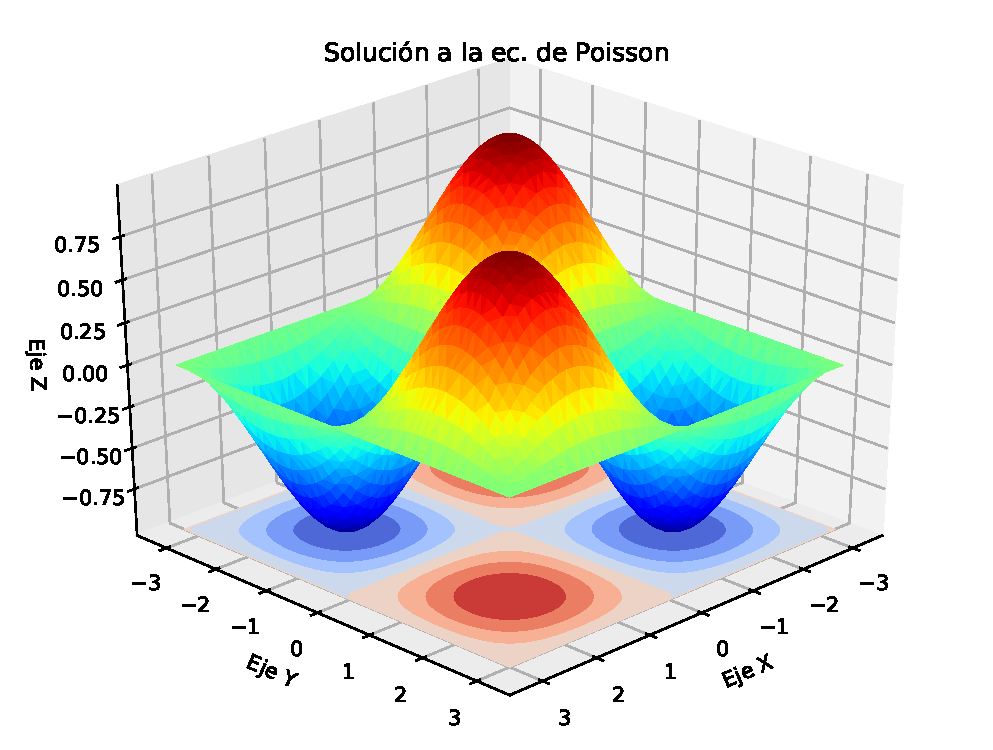
\includegraphics[scale=0.5]{Imagenes/Ejercicio_Ec_Poisson_01.eps}
   \caption{Gráfica de la solución a la ec. de Poisson.}
\end{figure}
\end{frame}
}
\begin{frame}
\frametitle{Elementos adicionales}
Como podrás ver, en la gráfica se agregó un mapa de contorno en la parte inferior de la gráfica, la función \funcionazul{tricontourf} es la que genera esa parte del gráfico.
\\
\bigskip
\pause
La gráfica obtenida es una buena aproximación a la solución exacta del problema.
\end{frame}
\begin{frame}
\frametitle{Elementos adicionales}
Para tener una idea general de la magnitud en la respuesta, podemos asociar una barra de color (\funcionazul{colorbar}) que determinar de manera autómatica el intervalo del valor, y le asocia el color de acuerdo al mapa de color elegido.
\end{frame}
\begin{frame}[fragile]
\frametitle{La barra de color}
En el mismo código para generar la gráfica, realiza las siguientes modificaciones:
\begin{lstlisting}[caption=Cambios en el código de la gráfica, style=FormattedNumber, basicstyle=\linespread{1.1}\ttfamily=\small, columns=fullflexible]
fig = plt.figure(figsize=(8,5))

surf = ax.plot_\textunderscore_trisurf(X, Y, Z, cmap=plt.cm.jet, lw=0.1)

fig.colorbar(surf, shrink=0.5, aspect=5)
plt.show()
\end{lstlisting}
\end{frame}
{\setbeamercolor{background canvas}{bg=white}
\begin{frame}
\frametitle{Gráfica obtenida}
\begin{figure}[h!]
   \centering
   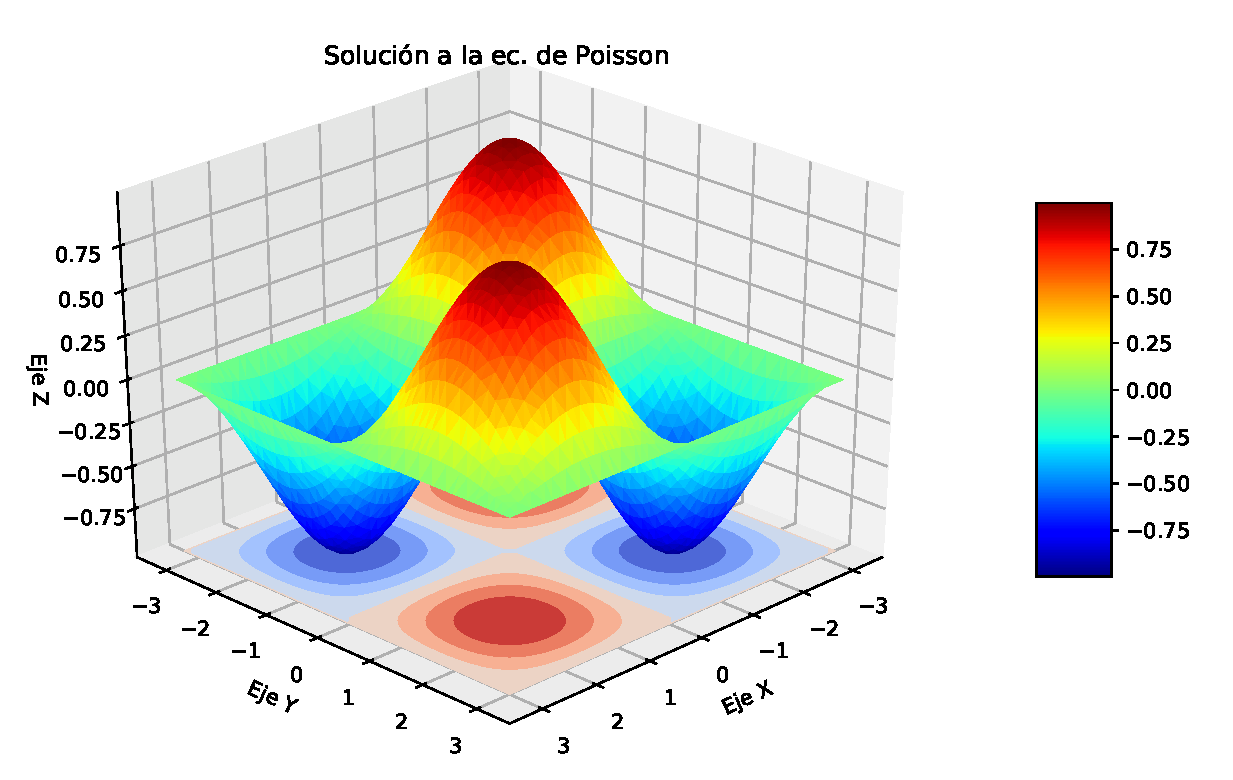
\includegraphics[scale=0.5]{Imagenes/Ejercicio_Ec_Poisson_02.eps}
   \caption{Gráfica con una barra de color incluida.}
\end{figure}
\end{frame}
}
\subsection{Dominios irregulares}
\begin{frame}
\frametitle{Dominios irregulares}
Cuando se trata de problemas para ecuaciones elípticas en dominios irregulares simplemente conectados (\emph{sin agujeros interiores}), una forma de describir los límites es delimitar los nodos interiores en una malla de discretización regular por un par de vectores, $\vb{i}_{\min}$ e $\vb{i}_{\max}$, cuyos componentes, $i_{\min}^{j}$ e $i_{\max}^{j}$, representan los índices $i$ que limitan en cada línea horizontal $j$.
\end{frame}
\begin{frame}
\frametitle{Dominios irregulares}
Para tales problemas, sin embargo, definir derivadas normales a los límites es bastante complejo.
\\
\bigskip
Por razones de claridad, acotamos la discusión a las condiciones de contorno de Dirichlet, que especifican los valores de la función en los límites inferior, izquierdo, derecho y superior:
\end{frame}
\begin{frame}
\frametitle{Condiciones de Dirichlet}
\begin{align}
\begin{aligned}
u_{i, 1}^{(r)} &= u_{i, 1}^{0}, \hspace{1cm} i = i_{\min}^{1}, \ldots, i_{\max}^{1}, \hspace{0.25cm} j = 1 \\[0.5em]
u_{i_{\min}^{j}, j}^{(r)} &= u_{i_{\min}^{j}, j}^{0}, \hspace{0.5cm} u_{i_{\max}^{j}, j}^{(r)} = u_{i_{\max}^{j}, j}^{0} \\[0.5em]
j &= 2, \ldots, N_{y} - 1 \\[0.5em]
u_{i, N_{y}}^{(r)} &= u_{i, N_{y}}^{0}, \hspace{0.25cm} i = i_{\min}^{N_{y}}, \ldots, i_{\max}^{N_{y}} \hspace{0.35cm} j = N_{y}
\end{aligned}
\label{eq:ecuacion_13_32}
\end{align}
\end{frame}
\begin{frame}
\frametitle{Ecuaciones a resolver}
En consecuencia, las únicas ecuaciones que deben iterarse para resolver tales problemas son las de los puntos interiores del dominio:
\end{frame}
\begin{frame}
\frametitle{Ecuaciones a resolver}
\begin{align}
\begin{aligned}
u_{i, j}^{(r)} &= \left[ k_{x} \left( u_{i-1, j}^{(r)} + u_{i+1, j}^{(r-1)} \right) + \right. \\[0.5em]
&\left. + k_{y} \left( u_{i, j-1}^{(r)} + u_{i, j+1}^{(r-1)} \right) - f_{i, j}  \right] / k_{x y} \\[0.5em]
i &= i_{\min} + 1, \ldots, i_{\max} + 1, \\[0.5em]
j &= 2, \ldots, N_{y} - 1
\end{aligned}
\label{eq:ecuacion_13_33}
\end{align}
\end{frame}
\begin{frame}
\frametitle{Malla de integración}
Se presenta a continuación un ejemplo de una malla de integración irregular y los índices de contorno por línea $i_{\min}^{j}$ e $i_{\max}^{j}$, para un dominio parecido a un disco.
\\
\bigskip
Los círculos negros representan los valores de contorno, los círculos blancos señalan los valores que deben de calcularse como solución.
\end{frame}
{\setbeamercolor{background canvas}{bg=white}
\begin{frame}
\frametitle{Malla de integración}
\begin{figure}[h!]
   \centering
   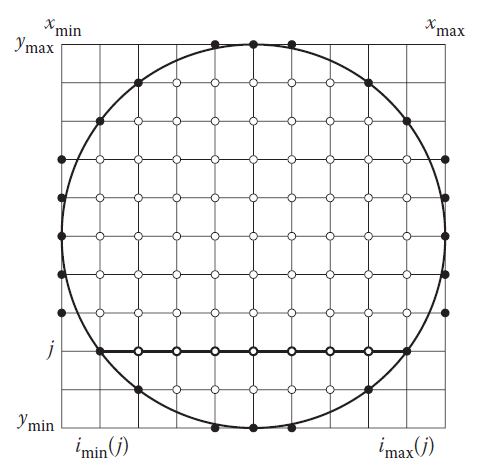
\includegraphics[scale=0.5]{Imagenes/malla_integracion_irregular_01.png}
   \caption{Malla de integración irregular.}
\end{figure}
\end{frame}
}
\begin{frame}
\frametitle{Código para la malla irregular}
La rutina que implementa el proceso iterativo para una malla irregular es \funcionazul{Poisson2D}.
\\
\bigskip
Las entradas de la función se describen a continuación:
\end{frame}
\begin{frame}
\frametitle{Código para la malla irregular}
Cuya entrada consiste en:
\setbeamercolor{item projected}{bg=blue!70!black,fg=yellow}
\setbeamertemplate{enumerate items}[circle]
\begin{enumerate}[<+->]
\item la aproximación inicial de la solución, recibida a través de la matriz \funcionazul{u} e incluye los valores de límite apropiados,
\item las coordenadas \funcionazul{x} e \funcionazul{y} de la cuadrícula de discretización,
\item las matrices con los índices de límites \funcionazul{imin} e \funcionazul{imax},
\seti
\end{enumerate}
\end{frame}
\begin{frame}
\frametitle{Código para la malla irregular}
\setbeamercolor{item projected}{bg=blue!70!black,fg=yellow}
\setbeamertemplate{enumerate items}[circle]
\begin{enumerate}[<+->]
\conti
\item el número de puntos de malla para las dos direcciones cartesianas, \funcionazul{nx} y \funcionazul{ny},
\item la precisión relativa requerida de los componentes de la solución \funcionazul{eps} y
\item el nombre de la función del usuario que evalúa el lado derecho de la ecuación de Poisson. 
\end{enumerate}
\end{frame}
\begin{frame}
\frametitle{Código para la malla irregular}
De manera similar a la función \funcionazul{PoissonXY}, la función \funcionazul{Poisson2D} realiza iteraciones de Gauss-Seidel para converger la solución \funcionazul{u} con la precisión deseada.
\end{frame}
\begin{frame}
\frametitle{Código para la malla irregular}
El refinamiento iterativo de la solución finaliza cuando el cambio relativo máximo de los componentes de la solución entre dos iteraciones consecutivas es menor que la tolerancia \funcionazul{eps}.
\end{frame}
\begin{frame}[allowframebreaks, fragile, plain]
\frametitle{Código \texttt{Poisson2D}}
\begin{lstlisting}[caption=Código para resolver un dominio irregular, style=FormattedNumber, basicstyle=\linespread{1.1}\ttfamily=\small, columns=fullflexible]
def Poisson_2_D(u, x, y, imin, imax, nx, ny, eps, Func):

   itmax = 10000

   f = [[0]*(ny+1) for i in range(nx+1)]

   hx = (x[nx] - x[1])/(nx-1); kx = 1e0/(hx*hx)
   hy = (y[ny] - y[1])/(ny-1); ky = 1e0/(hy*hy) 
   kxy = 2e0*(kx + ky)

   for j in range(2, ny):
      for i in range(2, nx): f[i][j] = Func(x[i], y[j])

   for it in range(1,itmax+1):
      err = 0e0
      for j in range(2,ny):
         for i in range(imin[j]+1,imax[j]):
            uij = (kx*(u[i-1][j] + u[i+1][j]) - f[i][j]) / kxy
            if (i >= imin[j-1] and i <= imax[j-1]): uij += ky*u[i][j-1] / kxy
            if (i >= imin[j+1] and i <= imax[j+1]): uij += ky*u[i][j+1] / kxy

            eij = 1e0 - u[i][j]/uij if uij else uij - u[i][j]
            if (fabs(eij) > err): err = fabs(eij)
            u[i][j] = uij

      if (err <= eps): break

   if (it >= itmax):
      print("Poisson_2_D: Se excedio el numero maximo de iteraciones !"); return 1
   return 0
\end{lstlisting}
\end{frame}
\subsection{Ejercicio dominio irregular}
\begin{frame}
\frametitle{Ejercicio en un dominio irregular}
Como ejercicio trabajaremos la ecuación de calor, para determinar la distribución de temperatura en un disco conductor, con condiciones de contorno: el semicírculo izquierdo del disco se encuentra a $\SI{100}{\degreeCelsius}$ y el semicírculo derecho está a $\SI{0}{\degreeCelsius}$.
\end{frame}
\begin{frame}
\frametitle{Ecuación a resolver}
En concreto, tendremos que resolver la ecuación de Laplace:
\begin{align}
\pdv[2]{u}{x} + \pdv[2]{u}{y} = 0
\label{eq:ecuacion_13_34}
\end{align}
en un disco circunscrito en un dominio cuadrado 
\begin{align*}
\mathcal{D} = [-a, a] \cp [-a, a]
\end{align*}
con $a = 5$.
\end{frame}
\begin{frame}
\frametitle{Condiciones de frontera}
Las condiciones de contorno son:
\begin{align}
\begin{aligned}
u_{i, 1}^{0} &= 0, \hspace{0.3cm} i = i_{\min}^{1}, \ldots, i_{\max}^{1}, \hspace{0.3cm} j = 1 \\[0.5em]
u_{i_{\min, j}}^{0} &= 100, \hspace{0.3cm} u_{i_{\max}, j}^{(r)} = 0, \hspace{0.3cm} j = 2, \ldots, N_{y} - 1 \\[0.5em]
u_{i, N_{y}}^{0} &= 0, \hspace{0.3cm} i = i_{\min}^{N_{y}}, \ldots, i_{\max}^{N_{y}}, \hspace{0.3cm} j = N_{y}
\end{aligned}
\label{eq:ecuacion_13_35}
\end{align}
\end{frame}
\subsection*{Código para el ejercicio}
\begin{frame}
\frametitle{Sobre el código}
Haremos algunas precisiones con respecto al código propuesto para resolver el ejercicio del disco y la ecuación de Laplace.
\end{frame}
\begin{frame}
\frametitle{Sobre el código}
En la implementación utilizaremos la función \funcionazul{FrontCondElipse} que puede manejar el caso más general de un \emph{dominio elíptico}, circunscrito por una cuadrícula cartesiana regular de tamaño $Nx \cp Ny$.
\end{frame}
\begin{frame}
\frametitle{Sobre el código}
Esta rutina determina los índices límite \funcionazul{ijmin} e \funcionazul{ijmax} en todas las líneas de cuadrícula horizontales de \funcionazul{Ny} y asigna los valores límite de la solución a los componentes apropiados de la matriz \funcionazul{u[][]}.
\end{frame}
\begin{frame}
\frametitle{Sobre el código}
La función \funcionazul{FrontCondElipse} en realidad no recibe la extensión geométrica del dominio de integración, y opera en cambio solo con los índices de nodos adimensionales, relacionando todas las posiciones con las coordenadas \funcionazul{x0} e \funcionazul{y0} del centro de la elipse adimensional.
\end{frame}
\begin{frame}
\frametitle{Sobre el código}
En cada línea de cuadrícula \funcionazul{j}, la rutina determina a partir de la coordenada \emph{y} relativa \funcionazul{yj} la intersección \emph{x} positiva con el límite elíptico, \funcionazul{xi} y, con ello, los índices delimitadores \funcionazul{imin[j]} e \funcionazul{imax [j]}. 
\\
\bigskip
\pause
Los valores límite de la solución se inicializan en función de estos índices de acuerdo con la ecuación (\ref{eq:ecuacion_13_35}).
\end{frame}
\begin{frame}
\frametitle{Sobre el código}
El programa principal es bastante similar al código usado para la solución de la ecuación de Poisson: básicamente inicializa las coordenadas de malla, marca los nodos exteriores con un valor distintivo, usa la rutina \funcionazul{FrontCondElipse} para establecer los valores límite, llama a la función \funcionazul{Poisson2D} para calcular los valores de la solución interior, y finalmente imprime la solución a un archivo de datos.
\end{frame}
\begin{frame}[allowframebreaks, fragile, plain]
\frametitle{Código completo}
\begin{lstlisting}[caption=Código para el ejercicio con dominio irregular, style=FormattedNumber, basicstyle=\linespread{1.1}\ttfamily=\small, columns=fullflexible]
from ModuloPoisson import Poisson_2_D

def Func(x, y):
   return 0e0

def FrontCondElipse(u, imin, imax, nx, ny):
   x_0_ = 0.5e0*(nx + 1e0)
   y_0_ = 0.5e0*(ny + 1e0)
   a = x_0_ - 1e0
   b = y_0_ - 1e0

   for j in range(1, ny+1):
      yj = j - y_0_
      xi = a * np.sqrt(1e0 - yj*yj/(b*b))
      if (xi == 0e0): xi = 0.75e0

      imin[j] = int(x_0_ - xi + 0.5e0)
      imax[j] = int(x_0_ + xi + 0.5e0)

   for i in range(imin[1], imax[1]+1): u[i][1] = 0e0
   for j in range(2, ny):
      u[imin[j]][j] = 100e0 * (nx - 2*imin[j])/(nx-1)
      u[imax[j]][j] = 0e0
   for i in range(imin[ny],imax[ny]+1): u[i][ny] = 0e0

a = 5
xmin = -a; xmax = a; ymin = -a; ymax = a
nx = 51; ny = 51
eps = 1e-5

u = [[0]*(ny+1) for i in range(nx+1)]
x = [0]*(nx+1); y = [0]*(ny+1)
imin = [0]*(ny+1)
imax = [0]*(ny+1)

hx = (xmax-xmin)/(nx-1)
for i in range(1,nx+1): x[i] = xmin + (i-1)*hx
hy = (ymax-ymin)/(ny-1)
for j in range(1,ny+1): y[j] = ymin + (j-1)*hy

for j in range(1,ny+1):
   for i in range(1,nx+1): u[i][j] = -1e99

FrontCondElipse(u,imin,imax,nx,ny)

for j in range(2,ny):
   for i in range(imin[j]+1,imax[j]): u[i][j] = 0e0

Poisson_2_D(u,x,y,imin,imax,nx,ny,eps,Func)

salida = open("DiscoLaplace.txt","w")
salida.write("x \t y \t u\n")
for j in range(1, ny+1):
   for i in range(1, nx+1):
      salida.write(("{0:10.5f} \t {1:10.5f} \t {2:14.5e}\n").format(x[i],y[j],u[i][j]))
salida.close()
\end{lstlisting}
\end{frame}
\begin{frame}
\frametitle{Gráfica obtenida}
El siguiente paso es representar la solución obtenida en una gráfica.
\\
\bigskip
En este caso, presentaremos una gráfica de contorno que indique el valor de temperatura dentro del disco circular.
\end{frame}
\begin{frame}
\frametitle{Gráfica obtenida}
La rutina de graficación es elaborada, pero cuentas con todo lo necesario para reproducirla.
\\
\bigskip
\pause
Verás que la aproximación a la solución es muy cercana a la solución analítica.
\end{frame}
\begin{frame}
\frametitle{Gráfica de contorno}
\begin{figure}[h!]
   \centering
   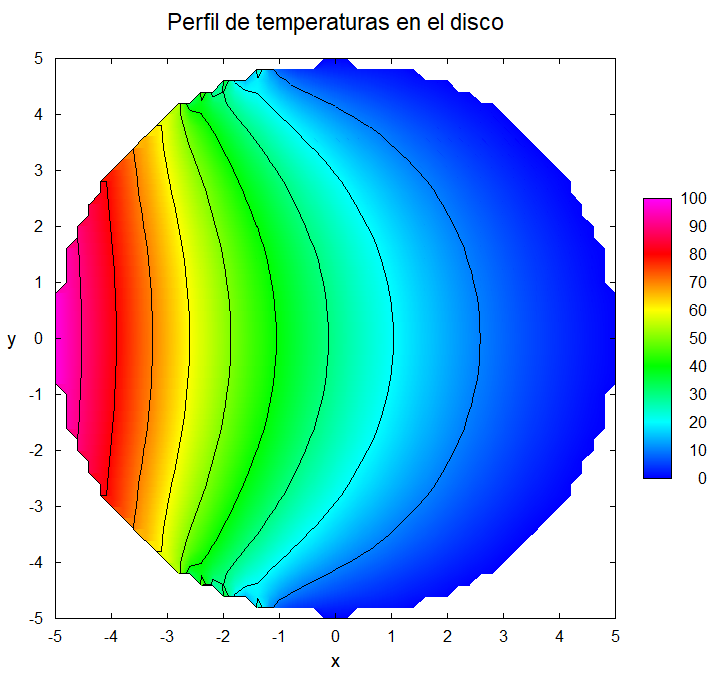
\includegraphics[scale=0.35]{Imagenes/ejercicio_Poisson2D_Plato_Circular_01.png}  
   \caption{Gráfica mostrando la solución a la ec. de Laplace.}
\end{figure}
\end{frame}
\end{document}
